\documentclass{tudelft-report}
\usepackage{amsmath}
\usepackage{graphicx}
\usepackage{subfig}
\usepackage{multirow}
\usepackage{pifont}
\usepackage{hyperref}
\usepackage{url}
\usepackage{pdfpages,caption}
\usepackage[toc,page]{appendix}
\usepackage{array}
\usepackage{blindtext}
\usepackage{wrapfig}
\usepackage[export]{adjustbox}
\usepackage{stackengine,graphicx}
\usepackage{graphicx,subfig}
\usepackage[export]{adjustbox}
\usepackage[parfill]{parskip}

\begin{document}

%% Use Roman numerals for the page numbers of the title pages and table of
%% contents.
\frontmatter

%% Uncomment following 19 lines for a cover with a picture on the lower half only
%\title[tudelft-white]{Title}
%\subtitle[tudelft-cyan]{Optional subtitle}
%\author[tudelft-white]{J.\ Random Author}
%\affiliation{Technische Universiteit Delft}
%\coverimage{cover.jpg}
%\titleoffsetx{10cm}
%\titleoffsety{10cm}
%\afiloffsetx{1cm}
%\afiloffsety{18cm}
%\covertext[tudelft-white]{
%    \textbf{Cover Text} \\
%    possibly \\
%    spanning 
%    multiple 
%    lines
%    \vfill
%    ISBN 000-00-0000-000-0
%}
%\makecover

%% Uncomment following 16 lines for a cover with a picture on the lower half only
\title[Literature Review]{Modelling the bicycle rider as a controller}
\author{C.\ Christoforidis}
\affiliation{Technische Universiteit Delft}
\coverimage{images/bike_rider.jpg}
\covertext{
    \textbf{Cover Text} \\
    possibly \\
    spanning 
    multiple 
    lines
    \vfill
    ISBN 000-00-0000-000-0
}

\makecover


%% Include an optional title page.
\begin{titlepage}

    \begin{center}
    
    %% Insert the TU Delft logo at the bottom of the page.
    \begin{tikzpicture}[remember picture,overlay]
        \node at (current page.south)[anchor=south,inner sep=0pt]{
            
\includegraphics{cover/logo}
        };
    \end{tikzpicture}
    
    %% Extra whitespace at the top.
    \vspace*{2\bigskipamount}
    
    %% Print the title in cyan.
    {\makeatletter
    \titlestyle\color{tudelft-cyan}\Huge\@title
    \makeatother}
    
    %% Print the optional subtitle in black.
    {\makeatletter
    \ifx\@subtitle\undefined\else
        \bigskip
        \titlefont\titleshape\LARGE\@subtitle
    \fi
    \makeatother}
    
    \bigskip
    \bigskip
    
    by
    %door
    
    \bigskip
    \bigskip
    
    %% Print the name of the author.
    {\makeatletter
    \titlefont\Large\bfseries\@author
    \makeatother}
    
    \vfill
    
    in partial fulfillment of the requirements for the degree of
    %in overeenstemming met de vereisten voor het verkrijgen van de graad van
    
    \bigskip
    \bigskip
    
    {\bfseries Master of Science}
    
    in Biomedical Engineering
    
    \bigskip
    \bigskip
    
    at the Delft University of Technology.
    %aan de Technische Universiteit Delft,
    
    %to be defended publicly on Tuesday January 1, 2013 at 10:00 AM.
    %in het openbaar de verdedigen op dinsdag 1 januari om 10:00 uur.
    
    \vfill
    
    \begin{tabular}{lll}
    %% Add additional information here, per faculty requirements, e.g
        Student number: & 4737822 \\
        Project duration: & \multicolumn{2}{l}{ 2018 -- 2019} \\
        Supervisor: & Dr.\ ir.\ A.L.\ Schwab, & TU Delft \\
        Thesis committee:
            & Dr.\ ir.\ R.\ Happee, & TU Delft \\
            & MSc.\ G.\ Dialynas, & TU Delft \\
    \end{tabular}
    
    %% Only include the following lines if confidentiality is applicable.
    \bigskip
    \bigskip
    \emph{This thesis is confidential and cannot be made public until May, 2019.}
    %\emph{Op dit verslag is geheimhouding van toepassing tot en met 31 december 2013.}
    
    \bigskip
    \bigskip
    \copyright2019\\
    C. Christoforidis\\
    ALL RIGHTS RESERVED
    An electronic version of this thesis is available at \url{http://repository.tudelft.nl/}.
    %Een elektronische versie van dit verslag is beschikbaar op \url{http://repository.tudelft.nl/}.
    
    \end{center}
    
    \end{titlepage}
    
    

\chapter*{Abstract}\label{chap:abstract}
\setheader{Abstract}

Bicycle riding is a fundamental part of everyday transportation in many countries around the world. Ever since the development of the safety bicycle, the bicycle remains  one of the most prominent means of transport. Despite cycling’s prominence in every day life for almost two centuries we still do not fully understand how the rider controls the bike in a more systematic way.

The purpose of this literature study is to explore and evaluate models of the single track vehicle rider found in the researched bibliography. Firstly a brief analysis of bicycle stability and its dynamics is presented as explored by Meijaard et al.\cite{meijaard2007linearized}. In Chapter \ref{results}models which were classified on their control theory approach are presented. In section \ref{ch:classical}, models using the classical control approach are described. Following the steps of early cybernetics research in which airplane pilot modelling was pioneered by McRuer\cite{mcruer1959human,mcruer1967manual,mcruer1967manual2}, a plethora of authors attempted adapting McRuers crossover model in order to model the rider of a seemingly much more complex task, motorcycle and bicycle riding. However some argued that such an approach will not work since cycling is not just a compensatory task. These spawned a new wave of research focusing in optimal control which is described in section \ref{ch:optimal}.  This approach has its roots in early motor control research in which the human brain is believed to work as a constrained optimal controller. In the final section of Chapter \ref{results}, all models that do not fall under the two approaches described above are reviewed. These include fuzzy logic controllers which have the advantage of incorporating heuristic  findings that are impossible to formulate using systematic mathematical approaches. Also intermittent control is briefly explored as a solution. 

Based on this literature review the graduation project will try to model the human controller for bicycles, while focusing  on the roll stabilization task. Open road experiments will be conducted in effort to estimate the controller’s parameters and indirectly validate it with real cycling data.



\begin{flushright}
{\makeatletter\itshape
    \@author \\
    Delft, April 2018
\makeatother}
\end{flushright}


\tableofcontents

%% Use Arabic numerals for the page numbers of the chapters.
\mainmatter

\chapter{Introduction}
\label{introduction}

Bicycle riding is a fundamental part of everyday transportation in many countries around the world. Ever since the development of the safety bicycle(two equal sized wheels, pneumatic tires, chain drive, rear wheel propulsion and a bent front fork), almost 130 years ago, the bicycle remains  one of the most prominent means of transport \cite{kooijman2013review}. With the growing concerns of sedentary lifestyles many choose the bicycle as their primary commute vehicle with the hopes of maintaining some levels of fitness. Additionally the bicycle is the preferred means of physical exercise for the elderly especially in the Netherlands and Denmark. Despite the fact that riding a bicycle is one of the first skills we acquire as kids and is used throughout the adult life, the fundamental way humans control the bicycle and ,generally single track vehicles,  is yet to be understood.\par
In a recent study examining the entries of patients to the emergency department due to traffic related accidents in the Netherlands (see Fig. \ref{fig:figure1}), it was found that bicycle related accidents were the most prevalent. With over 60,000 reported cases  bicycle accidents outnumber automobile accidents more than 4 to 1. It therefore  becomes clear that a lot could be done to improve cycling safety. Further look at the figure will reveal that most of those accidents did not involve a second party. There was  just a rider that fell off his bike. Although there are several potential reasons that riders lose control of the bicycle, formulating a general model of  how humans control single track vehicles could prove invaluable in understanding the causes behind the above numbers.

\begin{figure}[ht]
    \centering
    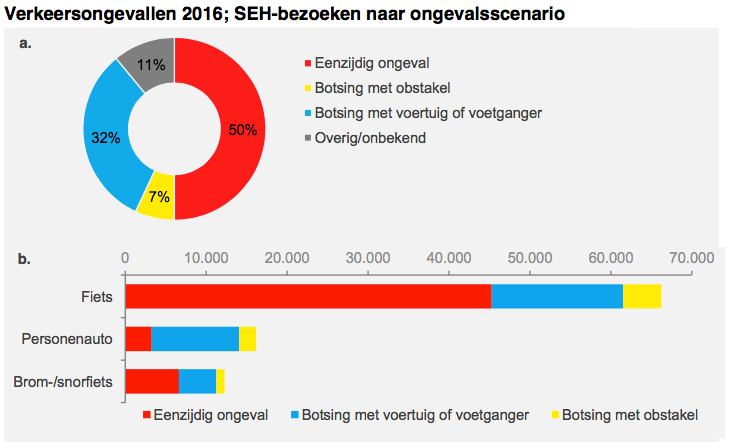
\includegraphics[scale=0.8]{images/figure1_1.png}
    \caption[Short title]{The number of road users that visit the emergency department at a hospital after a traffic accident in the Netherlands in 2016. Red indicates single vehicle accidents, yellow indicates a collision with an obstacle, blue indicates multi-vehicle accident and grey indicates other type of accidents\cite{krul_nijman_stam_2016}.}
    \label{fig:figure1}
\end{figure}

Following the steps of early cybernetics research in which airplane pilot modelling was pioneered by McRuer\cite{mcruer1959human,mcruer1967manual,mcruer1967manual2}, a plethora of authors attempted adapting McRuers crossover model in order to model the rider of a seemingly much more complex task; motorcycle and bicycle riding. However, some argued that such an approach will not work since cycling is not just a compensatory task. Moreover little concern was made to the fact that humans try to optmize for perfomance while simultaneously exerting the lowest amount of control effort. These spawned a new wave of research focusing in optimal control.  This approach is based in early motor control research in which the human brain is believed to work as a constrained optimal controller. 

A further look in motor control research will reveal the importance of the inernal model in control, state estimation and dead time compensation \cite{francis1976internal, garcia1982internal, wolpert1995internal, gillespie2016human}. The inernal model  theory argues that the motor system is controlled by the constant interactions between the process and the controller. In this case the process is the body, however in tasks like cycling the bicycle can be considered as an extension of the body. The internal model can be used either as a tool for control in the form of the inverse model \cite{edelmann2015,getz1995internal} or as a forward model in state estimation in combination with Kalman filters \cite{wolpert1995internal}. Additionally, forward models can be used in delay compensation algorithms \cite{miall1993cerebellum,van2001adaptive}. 

In this work an attempt to iterate over existing rider control models is made with the goal of answering two important questions. 
\begin{itemize}
        \item How signficiant is the effect of torque feedback for the balance task of bicycling?
        \item What is the prediction strategy best suitable for dead time  compensation in the balance task of bicycling?
\end{itemize}

In order to answer the above questions system identification techniques are employed using  the experimental dataset acquired within the scope of this thesis. In \cref{chapter2} an attempt is made to investigate the effect of haptic feedback in the task of balancing a bicycle under lateral perturbations. Non-parametric identification was conducted on the response of 20 riders in two different experimental conditions. In the first one the experimental bicycle operated as a normal bike while in the second the coupling between roll and steer was modified in order to cancel the torque feedback that would naturally transfer from the front wheel contact point to the handlebars. In \cref{hapticFB} further analysis is conducted by applying gray box identification techniques in order to investigate again the importance of torque feedback but also to test the effect of time delays in sensory feedback pathways and how these can be compensated throught the use of inernal model theory. In \cref{app:A,app:B,app:C} further details are presented on the methodology used to acquire proper measurments from the sensors of the experimental platform.


% Every human-machine system requires an understanding of how the plant operates. In the case of the bicycle multiple efforts have been made in capturing the dynamics of the bicycle and its  self-stabilizing behavior. These have resulted in a set of linearized equations of motion, now  commonly referred to as the Whipple Carvalho model \cite{meijaard2007linearized}, which is going to be discussed further in chapter \ref{results}.\par
% As it is known single track vehicles are not stable at low speeds. This is why a controller (like the human rider) is required to close the loop and create a stable system. There are two ways with which the human affects the dynamics of the plant. The first is with its passive interactions with the plant as a physical multibody system. Most passive models model the rider as a point mass rigidly attached to the rear frame, or as a pendulum connected to the rear frame \cite{eaton1975man}, although recent efforts have been made to extend this further with more complex passive rider models which include modeling of neuromuscular dynamics with spring-damper systems at various interfaces between rider and the bicycle frame\cite{dialynas2019}. The second is with its active control behavior. This involves the active control motion, such as steering, leaning or pedaling, applied by the rider to control and balance the bicycle. In most such cases, the passive behavior  of the rider is simplified by only  accounting for a fixed mass on the seat post, but when lean torque needs to be examined more complex modeling is required. The focus of the study is to explore the available models that best express the human rider as a controller in the bicycle-rider closed loop system.\par
% The literature review presented herein gives an overview of research done in the field of active rider modelling  concerning single-track vehicles, while discussing with which methods and to what extent have these models been validated. This extensive overview is given in section \ref{sub:rider} of chapter \ref{results}, which is structured in three sections: \ref{ch:classical} Classical control system design, \ref{ch:optimal} Optimal control system design and \ref{ch:other} Other control system design. Chapter \ref{conclusions} concludes on the results from Chapter \ref{results} having as a final goal to answer the research question:
% \par
% • \textbf{What is the controller that best simulates the behavior of the human in the control of single track vehicles?}


\chapter{Methods}
\label{methods}


In order to answer the research question posed, Google scholar was  used as the main tool of literature research. It proved to be the search engine with the most relevant and extensive literature.


In order to understand how a rider can be modelled as a controller, an understanding of single track vehicle dynamics is paramount. For that reason the first step was to seek literature that extensively describes the equations of motion of single track vehicles and analyses the unique problem arising from their inherent instability in low speeds. Search terms: “bicycle”, “dynamics”, “stability” , “motorcycle”, “equations + motion”, “eigenvalue + analysis”, “linear” , “non-linear”  were used.


\par
The next step was to find any published reviews on the subject of rider control for bicycles and motorcycles. The reviews of Kooijman et al.\cite{kooijman2013review}, Popov et al.\cite{popov2010review} and the bibliography review from Moore’s PHD thesis \cite{moore2012human} proved the most substantiated and extensive on the subject. A distinction was made between articles that were simply looking at bicycle and motorcycle control in general (ex. robot bicycles) and those that specifically tried to model the human controller. The latter  were more thoroughly visited. 

\par
In order to fill the gaps of more recent literature, an additional search on google scholar was conducted. The search was done by looking at papers involving keywords such as “rider control” , “rider identification” , “controller”, “optimal”, “McRuer”, “cybernetics”. For bicycle control results were filtered by looking at articles that directly cited the work of Meijaard et al. \cite{meijaard2007linearized} in bicycle dynamics, while for motorcycles results were filtered by looking at direct citations of Sharp’s work in motorcycle dynamics \cite{sharp1971stability}. These two articles involve the most prominent versions of linearized equations of motion for single track vehicle, so they are bound to be mentioned in any modern take on rider modelling.

Finally a search outside the scope of the problem was done looking at how the human controller is modelled in other motor related tasks. Search keywords included : “sensory-motor + integration” , “human + optimal + controller”, “Wolpert”, “Inverse + model”, “Internal + Model”, “feed-forward + control”.

All the relevant articles were stored in a database. If the article involved some form of control that the authour found unfamiliar, further research on the subject was conducted. These included fuzzy logic control, intermittent control and  model predictive control. After reading into the abstacts and conclusions of each article, an initial assesment was made on the relevancy of the work. Depending on that evaluation, a more extensive reading of the methods of some of the articles was done.
\chapter{Results}
\label{results}

\section{Bicycle dynamics and stability} \label{sub:bicycle}
This literature review aims to answer the research question regarding the validity of available rider models of single track vehicles. This includes both bicycles and motorcycles, as the list of bicycle rider models is not extensive enough. The plant is a necessary part of every closed loop control system and in this section the prevalent  way of expressing the dynamics and stability of a bicycle is described so as to better understand  what the controllers in the later sections are trying to actually control.
\subsection{The linearized Whipple-Carvalho bicycle model}
Bicycles are  very reliable transport vehicles and are considered the most efficient man powered form of transportation. Since the inception of the safety bicycle not much has changed with regards to the design of the two wheeled vehicle.   Bicycle design has been based on tinkering rather than equations which has resulted in little mathematical scrutiny in the available bicycle analyses. When trying to design a controller for a bicycle, a model that accurately describes its dynamics and kinematics is required but until 2007 there was no consensus on a set of equations that do that, so research on rider control for bicycles was hardly attempted. This changed when Meijaard et al.\cite{meijaard2007linearized}  developed a set of linearized equations of motion for the Whipple-Carvalho bicycle  model (fig \ref{fig:figure2}).\par
\begin{figure}[ht]
    \centering
    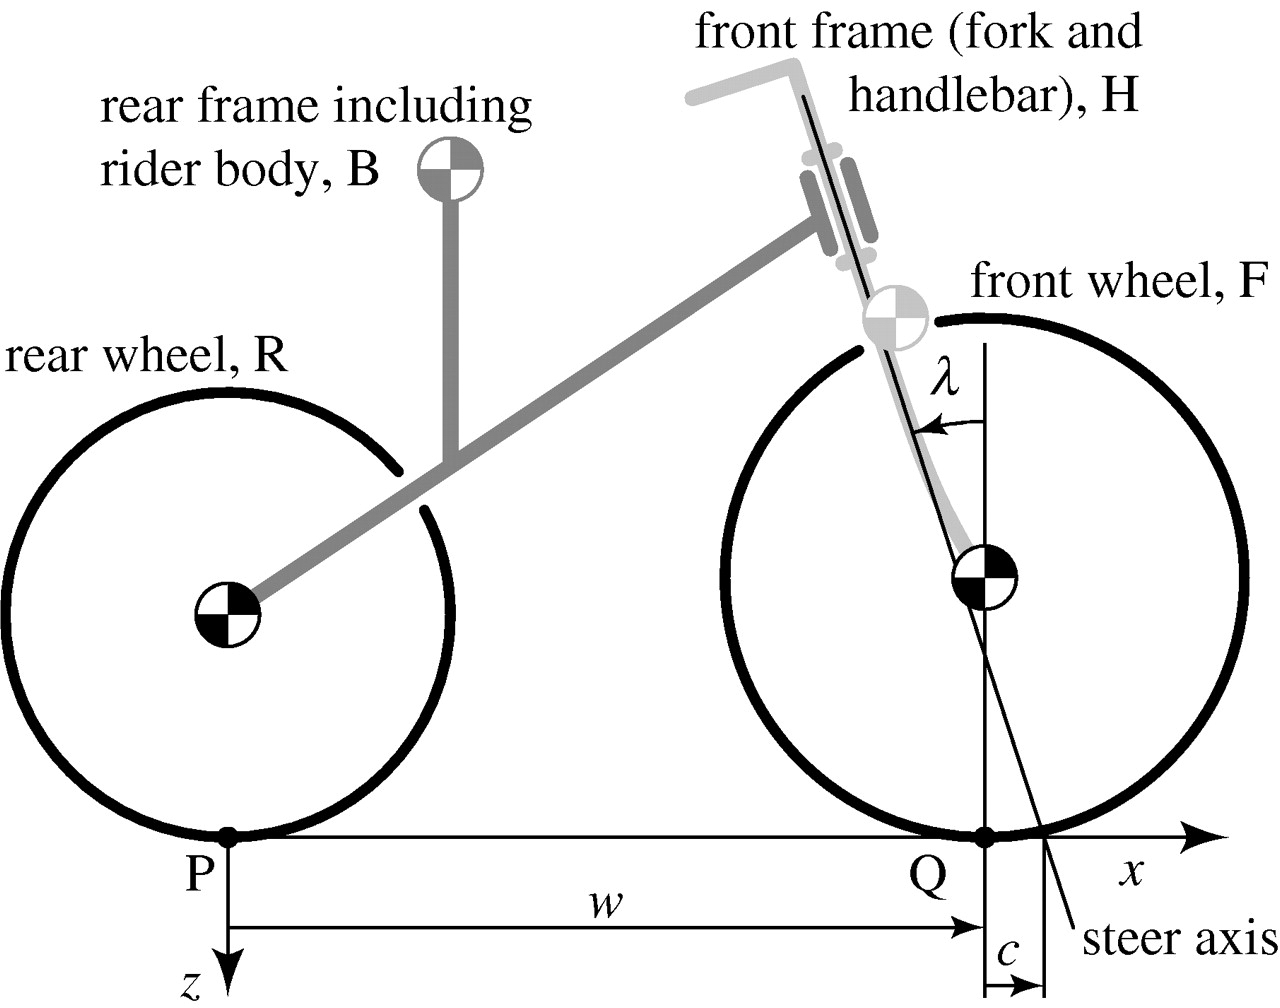
\includegraphics[scale=0.3]{images/figure3_1.png}
    \caption{ The Whipple-Carvalho bicycle model consists of four rigid bodies: rear wheel R, rear frame B, front frame H and front wheel F connected via hinges. The center of mass locations are expressed relative to the x - and z -coordinates shown (with origin at P and y pointing towards the reader). The other parameters shown are the steer axis tilt \ensuremath{\lambda}, wheelbase \ensuremath{w} and trail \ensuremath{c}. The model at its most expanded form is described by 25 parameters.\cite{meijaard2007linearized}}
    \label{fig:figure2}
\end{figure}


\vbox{%
    For  the equations of motion to be derived several assumptions were made by Meijaard  et al.\cite{meijaard2007linearized}:

    \begin{enumerate}
        \item The rider is rigidly connected to the rear frame with the mass of the arms included in the mass.
        \item The contact between tire and ground is modelled as a non-slipping rolling point-contact, meaning
              that wheels have an ideal rotation without lateral slip.
        \item Friction between moving parts and pedaling forces is neglected. Thus, the total energy of the
              system is constant.
        \item The bicycle is moving with constant forward velocity.
    \end{enumerate}}
\par
In order to understand the derived equations of motion a consideration must be made with regards to the configuration space and the velocity space of the model. The benchmark bicycle model derived is defined by 25 parameters. However, as a result of holonomic constraints (hinges and ground contacts) and non-holonomic constraints (non-slipping rolling contacts), its accessible configuration space can be reduced to 7 parameters. Coordinates \ensuremath{x_{P}} and \ensuremath{y_{P}} represent the translational position of the rear wheel point P, \ensuremath{\delta} is the steer angle, \ensuremath{\theta_{F}} and \ensuremath{\theta_{R}}  are the front and rear wheel angles respectively. Finally \ensuremath{\phi}  represents the lean angle about the x axis while \ensuremath{\psi}  represents the yaw rotation about the z axis. All this is depicted in figure \ref{fig:figure3}.
\begin{figure}[ht]
    \centering
    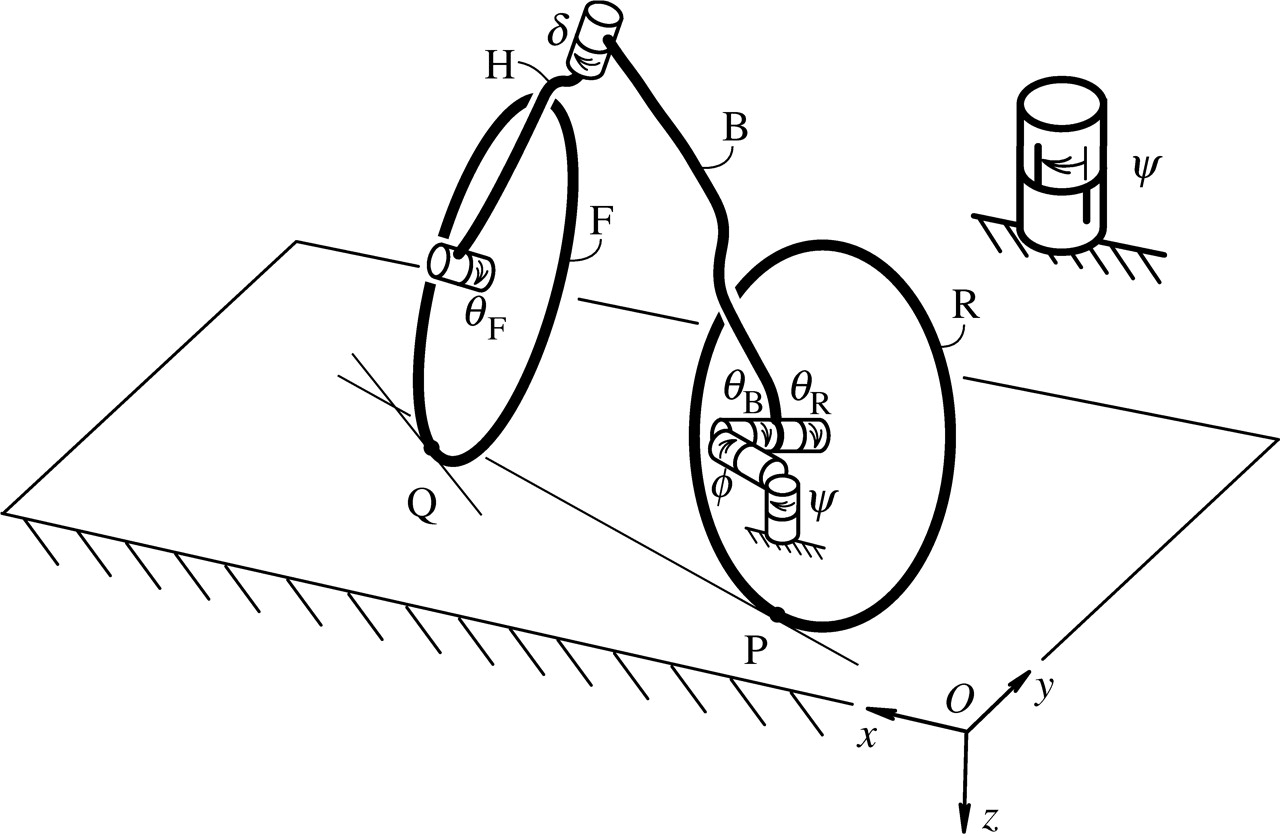
\includegraphics[scale=0.3]{images/figure3_2.png}
    \caption{Depiction of the benchmark bicycle in 3D. The cans represent a hinge between two rigid bodies. Multiple cans in series denote multiple degrees of freedom and the order of rotation.\cite{meijaard2007linearized}}
    \label{fig:figure3}
\end{figure}
\par
As it turns out some of the configuration variables do not appear in any of the equations of motion of the different parts. These so-called cyclic or ignorable coordinates are: the location of the bicycle on the plane (\ensuremath{x_{P}}, \ensuremath{y_{P}}), the heading of the bicycle \ensuremath{\psi} and the rotations (\ensuremath{\theta_{R}}, \ensuremath{\theta_{F}}) of the two wheels relative to their respective frames \cite{meijaard2007linearized}. Additionally due to a symmetry of the bicycle design and the lateral equations of motion, a  first order decoupling between forward and lateral dynamics exists \cite{meijaard2007linearized}. This means that the equations governing forward movement can be ignored when examining lateral dynamics like bicycle stabilization and vice versa. In conclusion, the three independent degrees of freedom that define the equations of motion are the  forward speed \ensuremath{\nu},  the lean angle \ensuremath{\phi} and the  steering angle \ensuremath{\delta} (figure \ref{fig:figure3}).
\subsection{The linearized equations of motion}
Keeping in mind the above considerations Meijaard et al.\cite{meijaard2007linearized} managed to formulate a set of three linearized equations that each describe a degree of freedom. The first is a first order differential equation that describes the forward speed as shown in equation \ref{eq:equation1}\cite{meijaard2007linearized}.
\begin{equation}
    \left[r_{R}^{2} m_{T}+I_{R y y}+\left(\frac{r_{R}}{r_{F}}\right)^{2} I_{F y y}\right] \ddot{\theta}_{R}=T_{\theta_{R}}
    \label{eq:equation1}
\end{equation}
where \ensuremath{I}, \ensuremath{r} and \ensuremath{m} denote inertia, radius and mass respectively of the rigid body defined in the subscript. Also \ensuremath{T_{\theta_{R}}} denotes the torque applied to the rear wheel in the direction of \ensuremath{\theta_{R}}.
\par
For the two remaining degrees of freedom the lean angle(\ensuremath{\phi}) and the steer angle (\ensuremath{\delta}) they found two second-order differential equations that are coupled and are given by equation \ref{eq:equation2}\cite{meijaard2007linearized}.
\begin{equation}
    \mathbf{M} \ddot{q}+v \mathbf{C}_{1} \dot{q}+\left[g \mathbf{K}_{0}+v^{2} \mathbf{K}_{2}\right] \mathbf{q}=\mathbf{f}
    \label{eq:equation2}
\end{equation}
where \ensuremath{q} is a vector containing the roll and steer angles, \ensuremath{f} is a vector containing the roll and steer torques, \ensuremath{g} is the gravitational acceleration and \ensuremath{\mathbf{M},\;v\mathbf{C}_{1},\;g \mathbf{K}_{0}+v^{2} \mathbf{K}_{2}} are the "mass", "damping" and "stiffness" ratios in matrix form respectively.

When talking about bicycle stability and control, equation \ref{eq:equation1} is often ignored as the task of pedaling is often removed from the problem so as to focus on pure roll stabilization. For control purposes it is convenient to express the bicycle equation \ref{eq:equation2} in state-space form . The state-space representation is:
\begin{equation}
    \dot{\mathbf{x}}=\mathbf{A} \mathbf{x}+\mathbf{B} \mathbf{f}
\end{equation}
\begin{equation}
    \mathbf{y}=\mathbf{C} \mathbf{x}+\mathbf{D} \mathbf{f}
\end{equation}
where matrices \ensuremath{A,B,C,D} are defined by:
\begin{equation}
    \mathbf{A}=\begin{bmatrix}
        -\mathbf{M}^{-1}v\mathbf{C}_{1} & -\mathbf{M}^{-1}(g \mathbf{K}_{0}+v^{2}\mathbf{K}_{2}) \\
        {\mathbf{I}}                    & {\mathbf{0}}
    \end{bmatrix} , \mathbf{B}=\left[ \begin{array}{c}{\mathbf{M}^{-1}} \\ {\mathbf{0}}\end{array}\right] ,
    \mathrm{C}=\begin{bmatrix} {\mathbf{0}} & {\mathbf{I}}
    \end{bmatrix} , \mathrm{D}=[\mathbf{0}]
\end{equation}
\par
By finding the eigenvalues of matrix \ensuremath{A} one can begin asking questions regarding the stability of the system. Meijaard et al. \cite{meijaard2007linearized} found the eigenvalues for different forwards speeds and managed to determine the region in which the uncontrolled benchamark bicycle was stable. In figure \ref{fig:figure4} the four eigenvalues are plotted in a forward speed range \ensuremath{0<v<10\; ms^{-1}}. The region that is defined when the real part of the weave eigenvalue becomes negative and the capsize eigenvalue has not crossed the zero threshold yet is the stable region and corresponds to forward speeds  \ensuremath{4.3\lessapprox v \lessapprox 6\; ms^{-1}}. When designing a controller  the input signals \ensuremath{f} are tasked with influencing the poles of the characteristic polynomial and moving the system from the unstable region to a stable one.

\begin{figure}[ht]
    \centering
    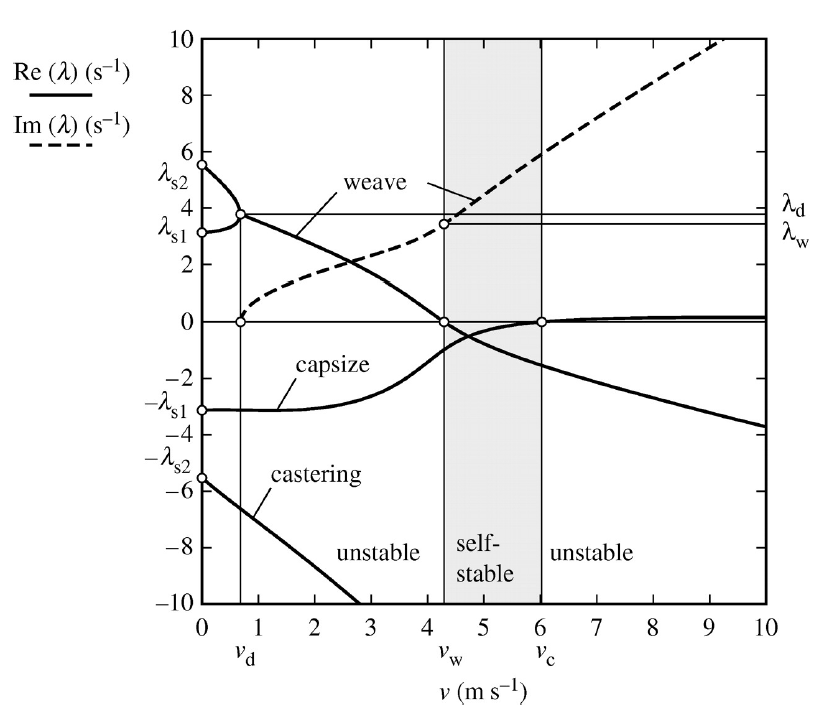
\includegraphics[scale=0.6]{images/figure3_3.png}
    \caption{Root locus plot of the benchmark bicycle. Bold black lines indicate the real part of the eigenvalues while dotted show the imaginary part.\cite{meijaard2007linearized}}
    \label{fig:figure4}
\end{figure}

Before exploring potential control options for the bicycle model described by the above equations, it is interesting to see to what extent is the model controllable. We know that the bicycles and motorcycles are controllable in reality but how well does this model capture reality is still a question.

To determine controllability of a dynamical system the reachability matrix :

\begin{equation}
    \mathbf{Q}=\left[\mathbf{B}, \mathbf{A B}, \mathbf{A}^{2} \mathbf{B}, \cdots, \mathbf{A}^{k-1} \mathbf{B}\right]
    \end{equation}
must be full rank. When the matrix rank is equal to the number of states of the system then the system is controllable by inputs \ensuremath{f}. By taking the determinant and then solving the equation:
\begin{equation}
    det\; \mathbf{Q} = \mathbf{0}
\end{equation} 
the forward velocities that result in an uncontrollable system can be found. Schwab et al. in \cite{schwab2010controllability} isolated the control inputs and found that a Whipple like bicycle with the an extended rider model can be controlled by either lean or steer torque for the practical range of 1 to 10 \ensuremath{\frac{m}{s}}. Although some forward speeds that result in a zero determinant exist they were either extremely close to zero or part of a stable mode so they concluded that they are of no concern.

\section{Rider modelling} \label{sub:rider}
When trying to model the rider of  single track vehicles some important considerations have to be made. As discussed in earlier sections the most important distinction comes from the consideration of which rider control inputs are implemented. When the focus of the model is purely on the steer control the rider body can be modelled as a simple fixed rigid body attached to the seat post of the vehicle as was implemented by Whipple \cite{whipple1899stability}. When the lateral body motion is considered significant control input, the rider  is often modelled as a two piece body. The lower part is still fixed on seat post but the upper part is modelled like an inverted pendulum. As a connection between the two, a spring dumper system is often placed \cite{aoki1999effectiveness,astrom2005bicycle,seffen1999bicycle}. The dynamics of  the combined system are expressed as extensions of the vehicle model.\par
Even when examining purely steer control, a distinction can be made between the types of control the rider performs, position(angle) or force (torque). For automobiles it is widely accepted that the driver controls the vehicle with position control \cite{plochl2007driver,guo1993modelling}. However for single track vehicles, where riders move the handlebars to a much lesser degree than in automobiles and where also the corner counter steer effect is present, a distinction cannot be easily made between which types of control the rider employs so models in literature  have explored both avenues.\par
The final important aspect that defines a rider model is the control task. For rider models of single track vehicles in literature, authors distinguish between  the stabilization task and the path following task.  Stabilization tasks  are used  when  trying to understand the effort applied by the rider in order to keep the vehicle from falling over. On the other hand  path following tasks are employed when the goal is to follow a set course. There are two types of models that are involved with path following tasks. The first is compensatory where the rider adjusts his position in order to minimize the difference between the refence trajectory and his current position. The second involves the concept of preview, this methods enhances the compensatory model by introducing a look ahead of the upcoming path. The decision at each moment is determined by a weighted average of the feedback and feedforward controller.

Given what was found in literature the controllers describing rider behavior were characterized by the above observations. This includes whether the model describes pure steer control (angle or torque) or implements some compensation for rider body dynamics. Also distinctions were made for models that tackled stabilization tasks or path following tasks. The models were also categorized depending on the underlying control theory  approach their authors employed. First there is the classical control approach which was most prominently applied to the airplane pilot behavior modelling. The second is the optimal control framework where the rider is assumed to be an optimal controller. This approach tries to introduce a weighted average between the effort put by the rider and the performance in the given task. Simulating the human controller as an optimal controller is a pathway that has been extensively explored in modelling of motor related tasks \cite{baron1984adaptive}. Finally all the rest were grouped under the banner of other methods. These include fuzzy logic, intermittent control, neural networks and controllers based on inverse dynamics.
\subsection{Classical control system design} \label{ch:classical}

The first attempt to model the human controller was done by McRuer for advancing the understanding of aircraft pilot control \cite{mcruer1967manual,mcruer1967manual2,mcruer1959human} in a post-war world where the study of cybernetics was blowing up. The general idea of the McRuer model is that the human controller tries to adapt so that the open loop system (fig.\ref{fig:figure5}) behaves like a first order integrator.
\begin{figure}[ht]
    \centering
    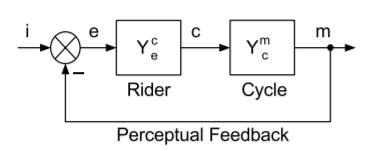
\includegraphics[scale=0.6]{images/figure3_4.png}
    \caption{Block diagram of a typical human-machine system control loop as described by McRuer, where \ensuremath{i} is the reference control value, \ensuremath{m} is actual control value; \ensuremath{e} is the control value error, \ensuremath{Y_e^c} is the human controller transfer function, \ensuremath{c} is rider output control variable and \ensuremath{Y_c^m} is the machine transfer function.\cite{kooijman2013review}}
    \label{fig:figure5}
\end{figure}
\par
For example if the pilot tries to control a task with first order dynamics (1st order integrator) then the human would act like a simple gain, leading to a first order integrator open loop system. McRuer found that this behavior is present for compensatory task in the vicinity of the gain cross over frequency, \ensuremath{\omega_c}. Cross-over frequency is the frequency that the open loop magnitude bode  plot crosses the unity line. He also introduced a time delay which comes from the inherent neuromuscular limitations of the human body. The formula for the open loop transfer function is shown below:
\begin{equation}
    Y_{e}^{c} Y_{c}^{m}=\frac{\omega_{c}}{j \omega} e^{-j \omega \tau}
    \label{eq:equation3}
\end{equation}
where \ensuremath{Y_e^c} is the pilot transfer function, \ensuremath{Y_c^m} is the transfer function describing the dynamics of the controlling task and \ensuremath{\tau} is the time delay. Equation \ref{eq:equation3} also known as the McRuer cross over model was enhanced to include further limitations of the human controller leading to equation \ref{eq:equation4} which is known as the McRuer precision model. This model makes the human a lead-lag system with time delay and limits the systems that a human operator can control.

\begin{equation}
    Y_{e}^{c}=K_{p} \frac{\left(T_{L} j \omega+1\right)}{\left(T_{I} j \omega+1\right)} e^{-j \omega \tau}
    \label{eq:equation4}
\end{equation}
where \ensuremath{T_L} is the time lead and \ensuremath{T_l} is the time lag.

\par
 The principles of this study were modified and implemented in numerous human controller modelling attempts for various tasks, from automobiles to tele-manipulators. Rider Models with the classical control approach were not deemed appropriate by many authors due to the multi loop control nature of single track vehicle stabilization and path following. This is why, not many of these types of models exist. However, recent attempts  by Hess\cite{hess2012modeling} and Schwab et al.\cite{schwab2013} have shown promising results.

\underline{\textbf{The Stasem and van Lunteren controller\cite{van1970influence}}}
\newline

Their model assumed angle control. It consisted of a PD controller with a time delay. The input was the frame roll angle and the output was the steer angle and upper body lean angle. They managed to get data for the system identification by creating a bicycle simulator. The goal of the study was to determine the effect of drugs on rider behavior by reflecting on the changes of the estimated parameters of the model. Unfortunately the experiments were conducted only on one speed (4.17 m/s) and the simulator provided no visual feedback. An interesting finding of this early study was the fact that path following and stabilization tasks did not seem to affect each other that much, as when the path following task was introduced  the proportional and derivative gains of the stabilization control loop did not alter significantly.

\bigbreak

\underline{\textbf{The CALSPAN group controller\cite{roland1971digital,roland1972bicycle,roland1973computer}}}
\newline

Following in Stasem’s and van Lunteren’s footsteps, Roland and Lynch developed a bicycle stability and path following controller but with the assumption that the output of said controller are torques, in comparison with the Delft model where angle control was assumed. The controller consisted of an inner loop which was responsible for stabilization and an outer loop which tried to minimize lateral deviation to achieve the tracking of a given trajectory.  The stabilization controller had the roll angle ,roll rate and roll acceleration as inputs  and consisted of a derivative, a proportional and an integral part (PID) with a time delay. The outputs were both the lean and steer torques. For the outer loop tracking controller, the input was the lateral deviation from the desired path and had an extra roll angle as output which was then added to the existing roll angle measured from the plant.  The only real experiments the model was used for were conducted by Rice\cite{rice1978rider} but the results did not compare well with the experimental data.

\bigbreak

\underline{\textbf{Weir’s rider model \cite{weir1973manual}}}
\newline

Weir developed a controller for Sharp’s motorcycle model\cite{sharp1985lateral} while being fully aware of McRuer’s prior work ,as he worked with him on many of his experiments. He assumed that torque control was far more plausible than angle control. His model is similar to the CALSPAN group model as it tries to tackle both stabilization and path following with lean torque and steer torque as plant inputs. However he tried to maintain single input single output transfer functions for his inner loops. He found from experimental data that  the best ones were the roll angle to steer torque due to the high gain and phase margins. His model is depicted in figure \ref{fig:figure6}. In contrast with the CALSPAN group controller Weir’s controller includes an additional  feedback loop for the control of the heading angle. The tracking controller output was also the heading angle and not the roll angle used by Roland et al.
\begin{figure}[ht]
    \centering
    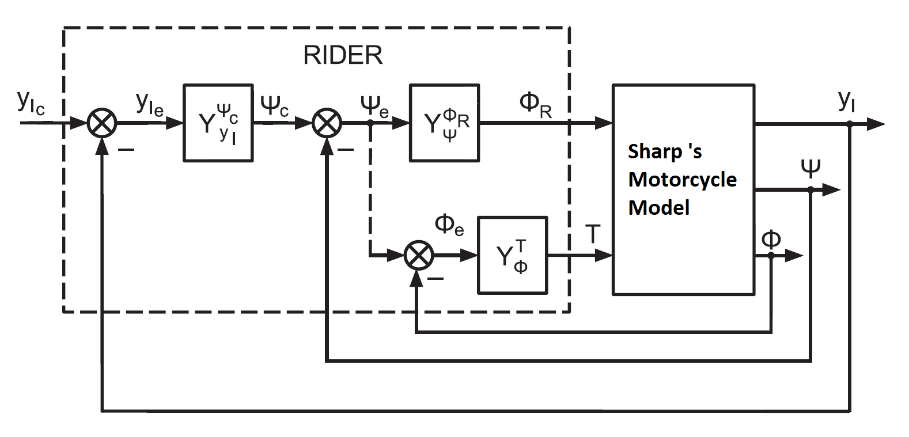
\includegraphics[scale=1.0]{images/weir_block.png}
    \caption{Weir's motorcycle rider model for Sharp’s motorcycle model. Plant outputs : lateral deviation (\ensuremath{y_l}), heading angle (\ensuremath{\Psi}), roll angle (\ensuremath{\Phi}),Rider controller inputs: plant ouputs ,reference path (\ensuremath{y_{l_c}}),Plant Inputs: steer torque (\ensuremath{T}), upper body lean torque (\ensuremath{\Phi_R}),  Trasfer Functions: tracking controller (\ensuremath{Y^{\Psi_C}_{y_l}}), heading controller  (\ensuremath{Y^{\Phi_R}_{\Psi}}), roll controller(\ensuremath{Y^{T}_{\Phi})})}
    \label{fig:figure6}
\end{figure}
\par
Eaton in his PHD thesis\cite{eaton1987man}  tried to validate the Weir model with experimental data. However he made some changes in order to get better results. Primarily he  focused on the inner roll stabilization loop and excluded the body lean torque as control input.
\par
Prem and Good\cite{prem1984rider} also worked with the Weir model in order to make observations about the steering behavior of novice motorcycle riders. In their experimental dataset they found that there is strong coupling between steering and rider upper body leaning inputs, so a modification was made on the Weir model introducing exactly that. They found that the extra coupling increases the gain of the transfer function allowing the large rider lean to roll angle error gain values to drop to more realistic levels. They also found comparable tracking capabilities with the stabilization ones and they concluded that although their model resulted in lower stability margins it resulted in far smaller upper body lean motions which in in experienced riders was always present.

\bigbreak

\underline{\textbf{Hess’s  rider model\cite{hess2012modeling}}}
\newline

In a recent attempt by Hess et al. to introduce a task independent handling qualities metric for bicycle control, he developed a model using the classical control approach. The behavior first observed by McRuer’s crossover model  can be captured by a variety of theoretical control structures from simple dynamics to complex neuromuscular models\cite{hess1984effects}. Hess believed that, the simpler models can often capture much of the essential dynamics in human-machine systems such as the bicycle-rider one. So he developed a model similar in nature to Weir’s and based on the foundation of the early McRuer experiments. The controller is using torque control and takes only the steer torque as input. More specifically, it has an inner roll stabilization loop, which can be seen in \ref{fig:figure7} ,and an outer heading and lateral deviation control  loop ,which is depicted in figure \ref{fig:figure8}.
\begin{figure}[ht]
    \centering
    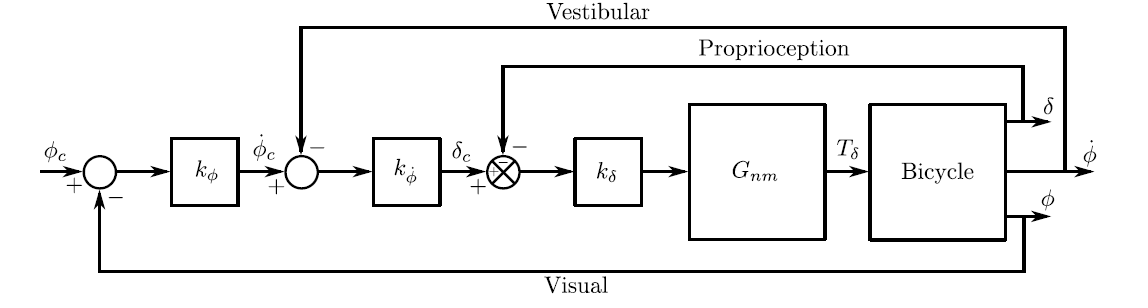
\includegraphics[scale=0.4]{images/hess_roll.png}
    \caption{The inner loop structure of the Hess Rider Controller with steer angle \ensuremath{\delta}, roll rate \ensuremath{\dot{\phi}}, and roll angle \ensuremath{\phi} feedback loops. The inner loops are closed with sequential gains starting with the proprioceptive steer angle loop, followed by the vestibular roll rate loop, and the visual roll angle loop. The steer angle loop captures the force/feel  we use while interacting with the handlebars.\cite{moore2012human}}
    \label{fig:figure7}
\end{figure}
\begin{figure}[ht]
    \centering
    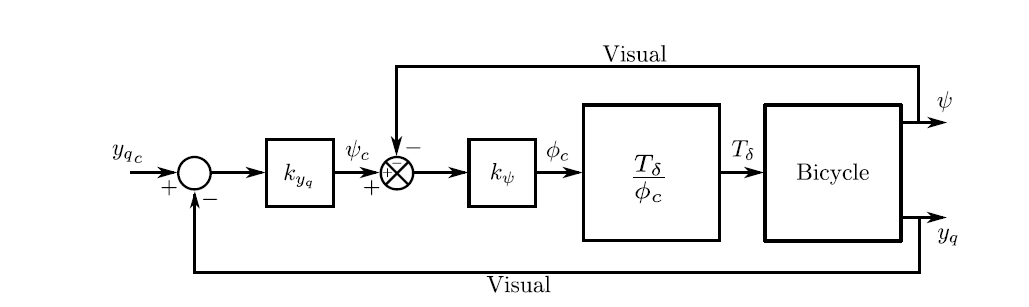
\includegraphics[scale=0.45]{images/hess_lat.png}
    \caption{The outer loop structure of the control system with the heading angle \ensuremath{\psi} and lateral deviation \ensuremath{y_q} being fed back.\cite{moore2012human}}
    \label{fig:figure8}
\end{figure}
\par
The model in essence contains five gain values for the five different feedback loops and two fixed second order filter coefficients determined by the neuromuscular system of the human along with a preview time parameter.  Although an attempt was made by Moore \cite{moore2012human} the model has yet to be experimentally validated.
\bigbreak
\underline{\textbf{The Schwab and de Lange model \cite{schwab2013}}}
\newline

First introduced in the master thesis of de Lange in 2011 and later published in 2014, this model is one of the most recent attempts to model the behavior of the bicycle rider which has been indirectly validated through system identification of its parameters. The particular model only examines the stabilization task and assumes  torque control. They also considered the upper body lean torque to be insignificant for stabilization purposes, so the only internal input of the plant was the steer torque. The input of the controller was the steer angle and roll angle of the bicycle. The controller consisted of a proportional, an integrative, a first- and a second-order derivative component acting on both the roll and steer angles (\ensuremath{K_\phi} and \ensuremath{K_\delta} respectively). While eight parameters were initially used they were later reduced by keeping only the ones that showed significant impact on the variance accounted for. This created a more realistic model of the rider and removed any potential concerns of overfitting the dataset. The controller is depicted in figure \ref{fig:figure9}.

\begin{figure}[ht]
    \centering
    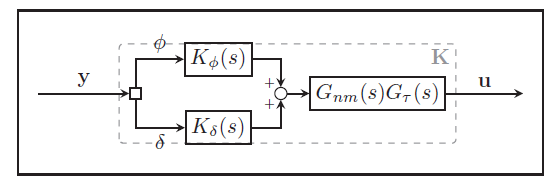
\includegraphics[scale=0.55]{images/deLange_block.png}
    \caption{Block diagram of the inner control structure of controller \ensuremath{K}, with roll and steering angle feedback gains \ensuremath{K_\phi} and \ensuremath{K_\delta}, time delay \ensuremath{G_\tau}, neuromuscular lag \ensuremath{G_{nm}}, input y (\ensuremath{\delta,\phi}) and output u (rider torque)\cite{schwab2013} }
    \label{fig:figure9}
\end{figure}

\par A second order filter was added in series to simulate the neuromuscular dynamics along with a time delay block. However the time delay was found to push the system to unstable regions and therefore was assumed to be zero.
\par
The Whipple model was enhanced by adding a lateral perturbation on the seat post as an external input. This was necessary in order to simulate the reaction of the rider model to an impulse response and make  the system identification possible. Firstly a non-parametric model was created by looking at the closed loop system as black box. This so called black box model was then used to evaluate the parametrized model described above. The gains were estimated by gradient descent optimization. What was found in the end was that some of the parameters could be omitted without significant drops of the variance accounted for. The four gains that remained were: the  gain on the lean angle and lean rate and the gain on the steer rate and the integral of the steer angle. The rider’s use of lean angle and lean angle rate represents vestibular and/or visual feedback, and the use of steer angle rate represents proprioceptive feedback. A major limitations in their experiments was the fact that they used data from cycling in a treadmill. This could very well have influenced the values of the gains estimated. However, further evaluation of this model with open road cycling experiments is planned.
\par
Finally the gains estimated were fed to an LQR model (will be discussed further in the next section) which was solved in an inverse manner in order to make an estimation of the control effort compared to the task performance for the particular stabilization task.

\begin{table}[tbp]
    \resizebox{\textwidth}{!}{\begin{tabular}{|l|l|l|l|l}
            \cline{1-4}
            \textbf{Models}                                                       & \textbf{Form of Control} & \textbf{Vehicle} & \textbf{\begin{tabular}[c]{@{}l@{}}Task (stabilizing or \\ path following)\end{tabular}} & \\ \cline{1-4}
            Stasem and
            van Lunteren \cite{van1970influence}                                  & Angle                    & Bicycle          & Stabilizing                         & \\ \cline{1-4}
            CALSPAN \cite{roland1971digital,roland1972bicycle,roland1973computer} & Torque (lean and steer)  & Bicycle          & Both                                & \\ \cline{1-4}
            Weir\cite{weir1973manual}                                             & Torque (lean and steer)  & Motorcycle       & Both                                & \\ \cline{1-4}
            Prem and Good \cite{prem1984rider}                                    & Torque (lean and steer)  & Motorcycle       & Both                                & \\ \cline{1-4}
            Hess \cite{hess2012modeling}                                          & Torque (steer)           & Bicycle          & Both                                & \\ \cline{1-4}
            Schwab \cite{schwab2013}                                              & Torque (steer)           & Bicycle          & Stabilizing                         & \\ \cline{1-4}
        \end{tabular}}
    \caption{Summary of all the rider models presented  from the classical control approach, classified according to form of control, vehicle type and control task.}
\label{table1}
\end{table}
\subsection{Optimal control system design} \label{ch:optimal}

Optimal controllers are a particular form of state feedback controllers where the parameters are determined through the minimization of a  cost function, which is a function of the state and the control variables. A general formulation of the cost function in continuous time is:
\begin{equation*}
    \min J(x_0,u)=\int_{0}^{T} F(x(\tau), u(\tau))d\tau
\end{equation*}
subject to the constraints below :
\begin{equation*}
    \frac{dx}{dt}=f(x,u) \; ,x(0)=x_0
\end{equation*}

\subsubsection{Linear Quadratic Regulator (LQR) Models}
The most widely used optimal controller is the linear quadratic regulator which can be used for MIMO systems described in state space form by :
\begin{align*}
    \dot{x}=Ax+Bu \\
    y=Cx+Du
\end{align*}
Where \ensuremath{x} is the state vector, \ensuremath{u} the control input, \ensuremath{y} the output vector. \ensuremath{A} is the system dynamics matrix, \ensuremath{B} is the input gain matrix, \ensuremath{C} is the observer matrix and \ensuremath{D} is the feedforward matrix.  A linear feedback control law of the form :
\begin{align*}
    u=-Kx
\end{align*}
is assumed with feedback gains \ensuremath{K} which are  determined by minimization of a cost function of the form:
\begin{align*}
    J=\int_{0}^{\infty} (xQx+uRu)dt
\end{align*}
where \ensuremath{Q} and \ensuremath{R} are the task performance coefficient matrix and the control effort coefficient matrix respectively. The solution of the matrix \ensuremath{K} is given by:
\begin{align*}
    K = R^{-1} B^T P
\end{align*}
where \ensuremath{P} is given by the algebraic Riccati equation:
\begin{equation*}
    A^{T} P+P A-P B R^{-1}B^{T} P+Q=0
\end{equation*}
A major disadvantage of this method is the fact that matrices \ensuremath{Q} and \ensuremath{R} need to be known beforehand and in most cases they are heuristically determined introducing subjective biases into the models.

\bigbreak
\underline{\textbf{Full state LQR controllers }}
\newline

Hubbard \cite{hubbard1979lateral} used the optimal control approach to create a model for skateboarding. He applied a full state feedback LQR for both the stabilizing and path following tasks for a skateboard. The human rider was modelled by body lean relative to the skateboard and the dynamics of the skateboard were neglected. The roll angle of the skateboard is taken as the control input. This model despite seemingly unrelated to single track vehicles paved the way for future attempts at modeling the bicycle rider as an optimal controller.
\par
Schwab et al.\cite{schwab2008some} created a similar controller as the one described above for the skateboard by Hubbard  but for the bicycle. The goal of the study was to determine the effect of upper body lean torque in the stabilization task in the control parameters. In the first model only steer control was assumed, which means that the dynamics of the rider were expressed as a simple fixed mass in the bicycle frame. They found that the bicycle is stabilizable with the LQR controller. However the roll angle feedback becomes unrealistically high for low speeds. In the second case the rider was modelled with an inverted pendulum for the upper body. They found that the eigenvalues and eigenmodes of the system remain relatively unchanged. However the gains for the upper body lean angle feedback gains were extremely high for low speeds even in the hands free situation where steer control is not a factor. They concluded that steer control is preferred by riders over body lean control when steering is possible.
\par
Connors and Hubbard \cite{connors2008modelling} also used a full state feedback LQR controller to model rider behavior but for a recumbent bicycle. They found that the oscillating legs can drastically increase the roll angle sensitivity and the steer torque required to balance the bicycle. Based on their findings they develop a control strategy that minimizes control effort for higher speeds.

\bigbreak
\underline{\textbf{Katayama LQR rider model \cite{katayama1988control}}}
\newline
\par
Katayama et al. developed a very extensive rider model for motorcycle control where they incorporated LQR control of the states along with a tracking with preview component, to investigate the behavior during LC maneuvers. The dynamics of the rider body was modelled as a double pendulum. The upper body was connected with the lower body which in turn was connected to the bicycle. Every hinge connection was modelled as a spring dumper system. The controller had only the roll angle as input from the states along with the average heading error. The controller outputs were the steer torque, the upper body lean torque and the lower body lean torque. What they concluded form their studies is that, for LC maneuvers, steering torque was dominant with lower body lean torque having an assistive role while the upper body lean torque does not contribute to the control that much.
\bigbreak
\underline{\textbf{Sharp’s preview model}}
\newline
\par
Sharp ,instead of simply feeding the state to an LQR optimal controller, incorporated a feedforward element to the model. The initial interpretation of the model was designed for cars and can been seen in figure \ref{fig:figure10}. Later he applied similar  models for motorcycles \cite{sharp2007motorcycle,sharp2006optimal} and bicycles\cite{sharp2008stability,sharp2007optimal}.
\begin{figure}[ht]
    \centering
    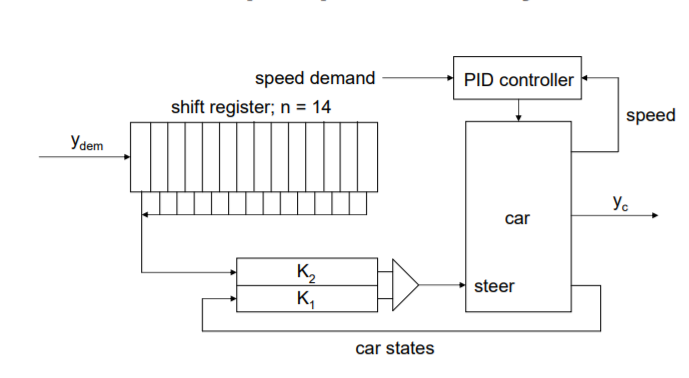
\includegraphics[scale=0.55]{images/sharp_model.png}
    \caption{Diagrammatic representation of a car tracking a roadway path at constant speed, with the whole system referenced to ground. Such a description implies that the road sample values pass through a serial-in, parallel-out shift register operation at each time step. \ensuremath{y_{dem}} is the previewable lateral displacement signal.\ensuremath{K_1} represents the full car-state feedback control, while \ensuremath{K_2} represents the preview control, in the form of feedback of the shift register states\cite{thommyppillai2009advances}. }
    \label{fig:figure10}
\end{figure}

The single track vehicle version of the model tackled the path following task and used torque control with both steer torque and body lean torque as  inputs to the plant. In order to incorporate the preview Sharp added to the traditional equations of motion of the plant, an additional set of equations, set in a ground based reference system, that took the form :
\begin{equation}
    \eta_{r}(k+1)=\mathbf{A}_{r} \eta_{r}(k)+\mathbf{B}_{r} \eta_{r n}(k)
\end{equation}
where \ensuremath{\eta_r} is the lateral displacement of the vehicle from the path at each moment while \ensuremath{\eta_{ri}} is the previewable lateral displacement which basically was  a sample from a white-noise random sequence. The length of the \ensuremath{\eta_r} signal was the preview length.\ensuremath{A_r} and \ensuremath{B_r} are sparse matrices of 1 and 0 that represent the road shift register process. Combining vehicle and road equations together, the full dynamic system is defined by :
\begin{equation}
    \left[ \begin{array}{c}{x_{v}(k+1)} \\ {\eta_{r}(k+1)}\end{array}\right]=\left[ \begin{array}{cc}{\mathbf{A}_{v}} & {0} \\ {0} & {\mathbf{A}_{r}}\end{array}\right] \left[ \begin{array}{c}{x_{v}(k)} \\ {\eta_{r}(k)}\end{array}\right]+\left[ \begin{array}{c}{\mathbf{B}_{v}} \\ {0}\end{array}\right] \boldsymbol{\tau}(k)+\left[ \begin{array}{c}{0} \\ {\mathbf{B}_{r}}\end{array}\right] \eta_{r n}(k)
\end{equation}
where \ensuremath{\tau} the plant input signal, \ensuremath{A_v} the vehicle dynamics and \ensuremath{x_v} the plant state.
\par

\begin{figure}[ht]
    \centering
    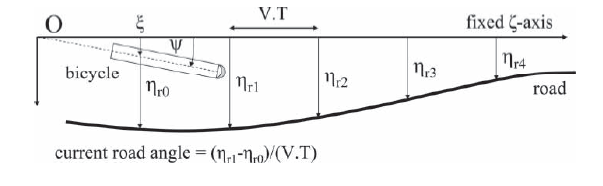
\includegraphics[scale=0.7]{images/sharp_preview.png}
    \caption{Illustration of the bicycle with speed \ensuremath{V} and discrete time interval \ensuremath{T} tracking a roadway in a ground-based reference frame\cite{sharp2007optimal}. }
    \label{fig:figure11}
\end{figure}
The cost function weighted the tracking errors for different preview lengths and the required control power. In the motorcycle studies \cite{sharp2007motorcycle,sharp2006optimal} they found that much larger preview distances were required compared to cars. However this has a hard cap at a certain point because the preview becomes so large that the gains associated with these preview points become zero. They also found a positive correlation between forward speed and preview distance. In the bicycle studies \cite{sharp2008stability,sharp2007optimal}  they found that the feedback gains are again  speed dependent but  become unrealistically high with reducing speed. Sharp concludes that the necessary preview time, as opposed to the motorcycle case, depends very little on speed. Finally he concludes that for precise control of a bicycle 2.5 seconds of preview are required for any given forward speed.
\subsubsection{Model Predictive Control Models}

The model predictive control problem (MPC) can be thought of as a repeated optimal control problem. Instead of finding and implementing the optimal control strategy by minimizing a cost function at time zero for a big optimization horizon, MPC is an iterative process where at each time step a new optimization problem is solved for a limited horizon. At each time step only the first control input result  of the optimization is implemented. In a algorithmic way MPC can be described from the steps below:
\begin{enumerate}
    \item At a sampling instant \ensuremath{t_k} obtain the state of the system to be controlled, i.e., \ensuremath{x(t_k)}.
    \item Solve the optimal control problem with initial condition \ensuremath{x(t_k) }over the \\  horizon \ensuremath{[t_k, t_{k+T}]} ,where \ensuremath{T} is the sampling horizon.
    \item Apply \ensuremath{u(t,x(t_k))} for t \ensuremath{\in [t_k,t_k+\delta)]}. Set \ensuremath{k \rightarrow k+1} and go to 1.
\end{enumerate}

\bigbreak
\underline{\textbf{Massaro's virtual rider model \cite{massaro2012virtual}}}
\newline
\par
Massaro et al. developed a virtual rider model for motorcycles. The virtual rider was designed to guide a continuous nonlinear  motorcycle model along generic target roll and target speed profiles. This implies that, in comparison with what is seen in all previous models thus far ,the rider model here is tasked to control the forward speed of the vehicle as well. At each time step an optimization problem is solved subject to the dynamics of  the plant for a limited horizon. Although  the plant model is non linear a technique was used where at each integration step the model was linearized around the equilibrium. The cost function weighted the tracking error and the input effort. The nonlinear control input which was used to guide the non linear motorcycle model was computed as  the sum of the linearized steady state component and a dynamic optimal component which they got from the optimization.
\par
They found a good comparison between  rider inputs(steering torque, rear wheel torque and front wheel torque) and real rider inputs despite the fact that upper body motions are not factored in the virtual rider model; which may affect performance of the controller in steep turns.
\bigbreak
\underline{\textbf{Chen and Chu MPC rider model \cite{chu2018modelling}}}
\newline
\par
Chen and Chu  developed a similar controller to Massaro based on model predictive control but for solving the roll stabilization task in a nonlinear bicycle model. They first used system identification to create a linearized prediction model from their non linear bicycle model. In order to do that simulations were made by controlling the nonlinear model with two PID controller; one for the lean torque and one for the steer torque. From the simulation data (torque signals and output signals), least squares regression was used to estimate the coefficients in the linearized mode’s matrices. This prediction model, along with a cost function, minimizing control inputs and tracking error, were used to get a valid input for the non linear bicycle model (see Fig.\ref{fig:figure12}).
\begin{figure}[ht]
    \centering
    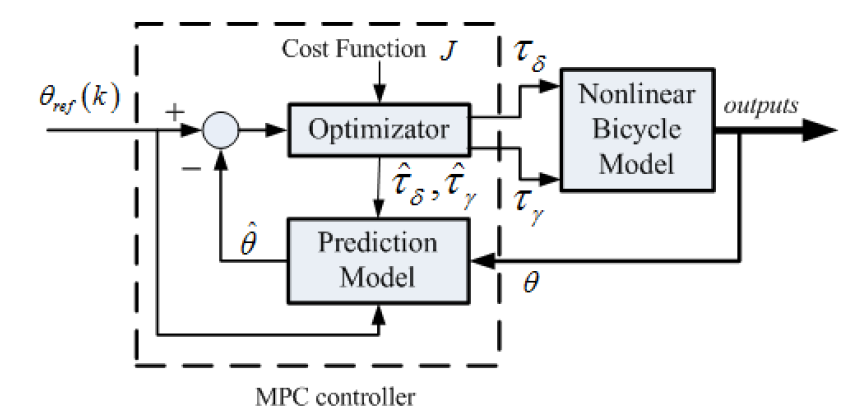
\includegraphics[scale=0.45]{images/chen_mpc.png}
    \caption{Block diagram of the Chen and Chu rider model, where \ensuremath{\theta} is the lean angle of the bicycle, \ensuremath{\tau_\gamma} is the upper body lean torque, \ensuremath{\tau_\delta} is the steer torque. The caret operator  indicates estimations made by the prediction module.\cite{chu2018modelling} }
    \label{fig:figure12}
\end{figure}
\par
The performance of their MPC controller was satisfactory but it has not been validated with experimental cycling data. Also a very strong dependency on the weighting matrices in the cost function was noted; which were estimated with trial and error and not through some systemic approach.

\subsubsection{\ensuremath{H_\infty} control models}

\ensuremath{H_p}control is a form of optimal control but with a particular form of optimization criterion explained below. One of the  most prominent implantation of \ensuremath{H_p} control uses the \ensuremath{l_\infty} norm and is called \ensuremath{H_\infty} control. The \ensuremath{l_\infty} norm is just the magnitude of the maximum element in a vector. For \ensuremath{H_\infty} control this involves finding  the supremum of the magnitudes  in the transfer function which has an external disturbance as input and the plant output as output. What it basically does is that it finds the gains that will result in a control signal that will minimize the effect of the external disturbance in the plant outputs.

\bigbreak
\underline{\textbf{Kamata and Nishimura model \cite{kamata2003system}}}
\newline
\par
They used \ensuremath{H_\infty} control to develop a roll stabilization controller for two identified motorcycle models. The first motorcycle model was fifth order and the second was third order. Both of their coefficients were estimated through system identification from experiments. The controller has the roll angle as an input and as an output the steer torque. No lateral body lean torque was incorporated. The controller was tested through simulations and not experiments. In order to verify the validity of the \ensuremath{H_\infty} controllers, the simulation results are compared with an uncontrolled case. They found that the controller of the 3rd order motorcycle model performed fairly well in comparison to the higher order dynamics model where stabilization performance was poor.
\bigbreak
\underline{\textbf{Mammar motorcycle rider model \cite{mammar2005motorcycle}}}
\newline
\par
Mammar et al. synthesized a steer torque controller using  \ensuremath{H_\infty} control to estimate the gains for roll stabilization of a motorcycle model. The roll angle was used as an input to the controller and the steer torque as output. The model also included feedforward capabilities. They ultimately found that the controller has good disturbance rejection and  handles cornering maneuvers well. However a forwards speed scheduling procedure was needed to handle forwards speed variations which was not implemented.

\begin{table}[ht]
    \centering
    \resizebox{\textwidth}{!}{\begin{tabular}{|l|l|l|l|l}
            \cline{1-4}
            \textbf{Models}                                                                              & \textbf{Form of Control} & \textbf{Vehicle}                                   & \textbf{\begin{tabular}[c]{@{}l@{}}Task (stabilizing or \\ path following)\end{tabular}} & \\ \cline{1-4}
            Full state LQR controllers \cite{hubbard1979lateral,schwab2008some,connors2008modelling}     & Torque (lean and steer ) & Bicycle (skateboard for \cite{hubbard1979lateral}) & Stabilizing                         & \\ \cline{1-4}
            Katayama's LQR model \cite{katayama1988control}                                                    & Torque (lean and steer)  & Motorcycle                                         & Both                                & \\ \cline{1-4}
            Sharp’s LQR model\cite{sharp2006optimal,sharp2007optimal,sharp2007motorcycle,sharp2008stability} & Torque (lean and steer)  & Motorcycle/Bicycle                                 & Both                                & \\ \cline{1-4}
            Massaro MPC model \cite{massaro2012virtual}                                                  & Torque (steer and wheel) & Motorcycle                                         & Both                                & \\ \cline{1-4}
            Chen and Chu MPC rider model \cite{chu2018modelling}                                         & Torque (lean and steer)  & Bicycle                                            & Stabilizing                         & \\ \cline{1-4}
            Kamata and Nishimura  \ensuremath{H_\infty} model \cite{kamata2003system}                                           & Torque (steer)           & Motorcycle                                         & Stabilizing                         & \\ \cline{1-4}
            Mammar  \ensuremath{H_\infty} model \cite{mammar2005motorcycle}                                                     & Torque (steer)           & Motorcycle                                         & Stabilizing                         & \\ \cline{1-4}
        \end{tabular}}
    \caption{Summary of all the rider models presented from the optimal control approach, classfied according to form of control, vehicle type and control task.}
\label{table2}
\end{table}
\subsection{Other control system design} \label{ch:other}

Below  rider models from literature are described,  that do not fall under neither the  category of classical control  or the optimal control banner.
\subsubsection{Fuzzy logic controllers}
A fuzzy logic control system is a control system based on fuzzy logic. Fuzzy logic refers to a mathematical system that analyzes analog inputs in terms of logical variables that take on continuous values between 0 and 1. This implies that expressions can take not only true or false  values like in normal computing  but also in between states. 
\par
Every fuzzy controller at a high level consists of four components shown in figure \ref{fig:figure15}. The Rule-base contains the sets of rules that describe how to best control the system. This may include if-else statements outlining the logic behind different decisions. The inference mechanism evaluates which of these rules are relevant at each moment and makes a decision on what the input to the process should be. The fuzzification interface simply translates the inputs to something that can be interpreted by the rules of the rule base. Finally the defuzzification interface coverts the conclusions reached to the inputs usable by the plant.

\begin{figure}[ht]
    \centering
    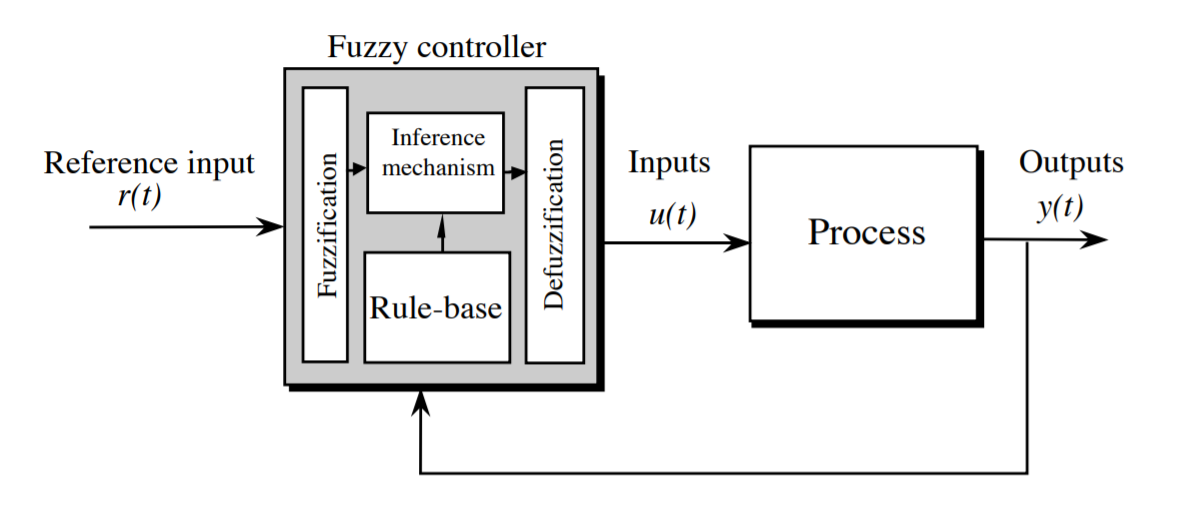
\includegraphics[scale=0.45]{images/fuzzy_controller.png}
    \caption{Fuzzy controller architecture \cite{Passino:1997:FC:550057} }
    \label{fig:figure15}
\end{figure}
\par
Fuzzy logic has the advantage that the solution to the problem can be cast in terms that human operators can understand, so that their experience can be used in the design of the controller. However many believe that fuzzy controller rely too heavily on unsubstantiated heuristics and ignore the importance of differential equations. Despite that fact fuzzy controllers can be useful when trying to simulate human behavior.

\bigbreak
\underline{\textbf{Chen and Dao fuzzy rider model \cite{chen2005dynamics,chen2006fuzzy,chen2007genetic}}}
\newline
\par
Chen and Dao  developed a bicycle controller using  fuzzy logic. The full model can be seen in figure \ref{fig:figure13}. The inner loop is responsible for roll balance and tracking of a reference roll angle. The outer loop is responsible for tracking a predetermined path. The controller output is the steer torque(\ensuremath{\tau_s}) while the input is the roll angle(\ensuremath{\theta}) and steer angle(\ensuremath{\delta}) for the inner loop and the heading angle (\ensuremath{\psi}), angle \ensuremath{\zeta} which is the difference between the path curvature and the heading angle, the coordinates of the vehicle and the coordinates of the orthogonal projection point of the vehicle center of mass to the curved path.
\begin{figure}[ht]
    \centering
    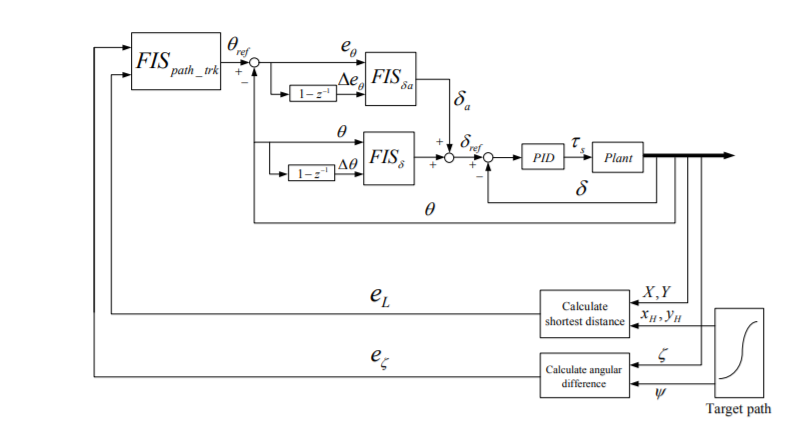
\includegraphics[scale=0.65]{images/dao_fuzzy.png}
    \caption{ Schematic block diagram of the full closed loop control system by Chen and Dao\cite{chen2007genetic}}
    \label{fig:figure13}
\end{figure}
\par
The PID controller shown generates the steer torque \ensuremath{\tau_s} using a reference steering angle(\ensuremath{\delta_{ref}} and the feedback steering angle from the plant. To generate appropriate  \ensuremath{\delta_{ref}}  a fuzzy controller (\ensuremath{FIS_{\delta}}) is used. It uses two inputs, the measured roll angle and its change (\ensuremath{\Delta\theta}). To achieve roll angle tracking another fuzzy controller is needed (\ensuremath{FIS_{\delta_\alpha}}). This controller uses as inputs the roll angle error (\ensuremath{e_\theta}) and its change (\ensuremath{\Delta e_\theta}) to generate appropriate output (\ensuremath{\delta_\alpha})) which in turn is added to the output of \ensuremath{FIS_{\delta}}. Finally to achieve path tracking a final fuzzy controller (\ensuremath{FIS_{path\_trk}}) is used with inputs the lateral deviation from the path (\ensuremath{e_L}) and the heading error (\ensuremath{e_\zeta}) and outputs the reference roll angle (\ensuremath{\theta_{ref}}). The parameters for all fuzzy logic controllers were estimated using genetic optimization. Good correspondence with simulation data was found from the controllers, but no validation with riding experiments was done.

\bigbreak
\underline{\textbf{The Sergey and Fjii fuzzy controller\cite{sergey2004model}}}
\newline
\par
Fujii and the Sergeys also developed a controller for a scooter to model roll stabilization and path tracking using fuzzy control. They used steer control with a PD controller operating under feedback from the roll angle. The reference roll angle signal was computed using the fuzzy controller similar to the way explained in the Chen and Chao model. A genetic algorithm was used to minimize a fitness function in order to estimate the fuzzy controller parameters.  In their experimental validation they found that estimated state signals showed good match but the steering torque not so much. Again no validation with experimental data was done.

\subsubsection{Inverse dynamics rider models}
Inverse dynamics are used to determine the forces required to pursue a desired course based on the current state. In motor control studies, inverse models are often used to simulate the process of learning. As the user becomes more experienced with a task his internal model of the process he is trying to control gets better. This allows the user to rely much less on sensory feedback which is inherently restricted by neuromuscular dynamics and neural time delays. This internal model is often represented as an inverse model of the plant dynamics. 

\bigbreak
\underline{\textbf{The Getz rider model\cite{getz1995internal,getz_marsden}}}
\newline
\par
Getz developed and inverse dynamics methods he calls dynamic inversion which he applied to bicycle control. In his approach the plant model output which could be either the roll angle or the later deviation is fed into an inverse prediction plant model which will give an appropriate steer torque as output. Such a model shows great promise for determining the performed control by a rider based on a traversed path ,but its performance is questionable for the case where the path is roughly described; which is much more realistic for modeling real rider behavior.

\bigbreak
\underline{\textbf{Edelmann rider model\cite{edelmann2015}}}
\newline
\par
In this work Edelmann et al. combined the approaches of classical control with that of the inverse dynamics models to create the bicycle rider model depicted in figure \ref{fig:figure13}.
\begin{figure}[ht]
    \centering
    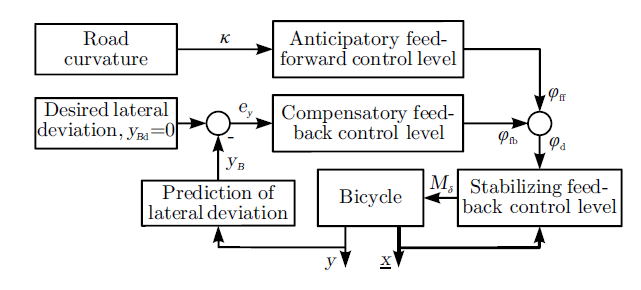
\includegraphics[scale=0.65]{images/edelmann_hybrid.png}
    \caption{Block diagram of the controller architecture by Edelmann et al. The anticipatory feed forward control level produces the roll angle (\ensuremath{\phi_{ff}}) which is combined with the output of the compensatory controller (\ensuremath{\phi_{fb}}) to produce the reference roll angle (\ensuremath{\phi_d}) which is fed to the inner stabilizing feedback control level which in turn produces the steer torque input to the plant (\ensuremath{M_\delta}). \ensuremath{y} is the positional output of the bicycle which passes through the prediction module to get the lateral deviation (\ensuremath{y_B}). \ensuremath{\kappa} is the curvature signal of the route and \ensuremath{\underline{x}} is the state of the bicycle.\cite{edelmann2015} }
    \label{fig:figure14}
\end{figure}
The model employs steer control and tackles both stabilization and path tracking tasks. It consists of three distinct parts. The stabilizing feedback controller is a state feedback controller similar to the one described by Hess \cite{hess2012modeling} and its purpose is to stabilize potentially unstable modes of the bicycle. Instead of getting the full state  from the plant, the roll angle is further processed by the compensatory feedback and anticipatory feedback controllers which is then fed back into the inner loop. The Anticipatory feedforward controller is responsible for modelling the rider behavior regarding the trajectory ahead. Roll angle \ensuremath{\phi_{ff}} is determined by combining an inverse model of the plant and a formula which models the anticipatory behavior of the rider depending on the curvature at the preview points. The outer loop responsible for compensatory feedback tackles the reactionary rider behavior regarding the path following task. In this controller the output  of the plant model is fed again to an inverse prediction model where the later deviation of the next time step  is outputted. This lateral deviation error (\ensuremath{e_y}) is fed to the compensatory feedback controller which is basically the precision model expressed by McRuer (see \ref{eq:equation4}).
\par
In their simulation results they found that the stabilizing feedback control level stabilizes the demanded roll angle with little time delay. However the demanded steady state roll angle was not reached. They attributed this to the fact that  the model does not display the self-adaptation principle of its internal inverse model; behavior that is prevalent in all motor tasks which involve a learning process.
\subsubsection{Intermittent Control System Design}

Intermittent control is a feedback control method which provides a spectrum of possibilities between the two extremes of continuous-time and discrete-time control. Conventional sampled-data control uses a zero-order hold. In contrast to conventional sampled data control, intermittent control explicitly embeds the underlying continuous-time closed-loop system in a system-matched hold which generates an open-loop intersample control trajectory based on the underlying continuous-time closed-loop control system. This approach has been recently documented by Gawthrop et al. \cite{gawthrop2014intermittent} where they modified the observer, predictor, state-feedback (OPF) model ,developed by Kleinman  \cite{kleinman1970optimal}, by transforming the continuous time state feedback to feedback in intermittent time. In physiological terms, they  described their approach to human motor control as “continuous observation, intermittent action”.

\bigbreak
\underline{\textbf{Doyle rider model\cite{doyle1988}}}
\newline
\par
Intermittent control has also been applied in bicycle rider modelling by Doyle. Doyle used bicycle stabilization observations to develop a bicycle rider model for roll stabilization. He ended up using steer torque control with continuous feedback on the roll rate ,acceleration and intermittent feedback on the roll angle. The intermittent feedback is activated when the roll angle error exceeds a certain threshold which he found to be \ensuremath{1.6^o}. Doyle used this model to investigate to what extent motor skills involve higher cerebral functions. In order to this he used this model in two experimental set ups. In the first one he used a normal bicycle while in the second he used a special ‘destabilized’ bicycle where factors such as gyro, trail and head-angle had been removed. With the second experimental setup he found that the steering signals follow the roll signals with a mean 120 ms delay. He concluded that the system delay in the roll angle rate is so short that  the output from the vestibular system must go directly to the controlling muscles bypassing higher cortical function.

\begin{table}[ht]
    \centering
    \resizebox{\textwidth}{!}{\begin{tabular}{|l|l|l|l|l}
            \cline{1-4}
            \textbf{Models}                                                                              & \textbf{Form of Control} & \textbf{Vehicle}                                   & \textbf{\begin{tabular}[c]{@{}l@{}}Task (stabilizing or \\ path following)\end{tabular}} & \\ \cline{1-4}
                Chen and Dao fuzzy rider model \cite{chen2005dynamics,chen2006fuzzy,chen2007genetic}     & Torque (steer) & Bicycle  & Both                        & \\ \cline{1-4}
                Sergey and Fjii fuzzy controller \cite{sergey2004model}                                                    & Torque (lean and wheel)  & Motorcycle                                         & Both                                & \\ \cline{1-4}
                Getz inverse dynamics model\cite{getz1995internal,getz_marsden} & Torque (steer)  & Bicycle                                 & Both                                & \\ \cline{1-4}
                Edelmann inverse dynamics model\cite{edelmann2015}                                                  & Torque (steer) & Motorcycle                                         & Both                                & \\ \cline{1-4}
            Doyle intermittent control model \cite{doyle1988}                                         & Torque (steer)  & Bicycle                                            & Stabilizing                         & \\ \cline{1-4}
      
        \end{tabular}}
    \caption{Summary of all the rider models presented using fuzzy control ,inverse dynamics and intermittent control, classified according to form of control, vehicle type and control task.}
    \label{table3}
\end{table}



\chapter{Conclusions}
\label{conclusions}

Weir wrote in his original paper in 1979 "The presence of a human operator as the controller places additional constraints on the control situation. He is limited in his ability to sense feedback cues and in the rapidity and precision with which control actions can be made.". Designing a human controller for any motor related task is not as simple as plugging a controller and solving an optimization problem or placing poles in the stable region. 
\par
Multiple considerations must be made for the human as physiological system. What was made clear from the start of cybernetics research is that neuromscular dyanmics should be somehow accounted for. In \cite{hess2012modeling,schwab2013,moore2012human} the neuromuscular dynamics were modeled as a mass spring damper system with predermined coefficients. Considering all the information gathered from previous attempts in modelling the human rider in single track vehicles, it is evident that when designing a human controller the system's feedback loops should have a correspondence with the human's own sensory feedback systems. It is known that when riding a bicycle or a motorcycle visual, proprioceptive  and vestibular feedback work together to give our cortex an estimation of the state of the vehicle we are controlling. In  \cite{hess2012modeling,schwab2013,moore2012human} it is made clear that proprioceptive feedback is linked with steer angle and steer rate feedback, which makes sense since the muscle spindles in our hands that are touching the handlebars should give us information on its perceived location and motion. As far as our perception of roll is concerned the vestibular and visual system  are involved. Hess et al.\cite{hess2012modeling} attributed roll rate feedback to the vestibular and the roll angle feedback to visual. Finally for the path following task, heading and lateral deviation changes are perceived  through our visual system (see Fig. \ref{fig:figure8}).

Another major consideration with human control of single track vehicles is the fact that the task is not entirely compensatory. Especially in the path following component preview plays a very significant role. This was explored extensively by Sharp \cite{sharp2007motorcycle,sharp2006optimal,sharp2008stability,sharp2007optimal,thommyppillai2009advances}. Another consideration is the human's ability to learn through the creation of internal models. It is a prelevant theory in motor control research that humans, for every motor related task, have an internal model of each process that estimates the state of the system. The internal model estimation is then fused with the delayed senosory feedback pathways resulting in more accurate and faster estimations of the state \cite{wolpert1995internal}. What makes it even more complicated is the fact that this internal model is dynamically changing. It changes as the human's experience with the task improves. Prem and Good \cite{prem1984rider} in their studies explored the effects of riding experience and found that lean body motions are less and less prevalent the more experienced the rider becomes, so the human operates on pure steer control. Edelmann et al.\cite{edelmann2015} incorporate an anticipatory feedforward level to their control architecture in order to counter the effects of the inherently delayed compensatory feedback control level.

The rider models of table \ref{table2} all fall under the umbrella of optimal control. These authors made the assumption that humans when trying to control single track vehicles operate as constrained optimal controllers, which is not that far fetched to believe considering past research on motor control \cite{wolpert2007probabilistic}. In \cite{chu2018modelling,massaro2012virtual},  the authors went a step further by  introducing the concept of MPC, which again comes back to the way our eternal shifting brain functions operate. One would not expect the brain to compute the optimal solution at time zero and then operate under the assumption that its initial computation is 100\% correct. A more reasonable approach would be a process in which our brains adapt and respond by computing optimal scenarios throughout the execution of the task. This is exactly what the MPC models are trying to simulate.

There is no "best" approach when considering the fact that a lot of models are trying to tackle different control tasks. A controller looking at pure stabilization will look different than one that tries to simulate the whole riding behavior from path following to roll stability. What makes the single track vehicle problem unique is their inherent instability at speeds outside the stable region. Design and validation of stabilization controller should be first priority.  While it has not been systematically proven the preferred method of control for the majority of the literature explored seems to be torque control (see tables \ref{table1}, \ref{table2}, \ref{table3}).Also worth noting is the fact that lean torque is often deemed insignificant especially in controllers where roll stabilization is the controlling task \cite{katayama1988control,van1970influence,hess2012modeling,schwab2013}. The importance of proprioceptive feedback in these must not be understated.

In conclusion complex controllers that tackle multiple tasks in multiple nested control loops are very hard to be validated with experiments so they will not be part of the focus of my research going forward. My aim wil be to implement a rider model similar to the Schwab and de Lange model \cite{schwab2013} that can be indirectly validated, throught system identification of its parameters in open road riding experiments.


%% Use letters for the chapter numbers of the appendices.
\appendix

%
\chapter{Calibration of Inertial Measurements} \label{app:A}

The fixed body angular velocities measured by the Inertial Measurement Unit (IMU) are biased due the imperfect orientation of the sensor axis (see \cref{fig:bike_imu}). The goal is  it to allign system xyz with the global coordinate system XYZ. To achieve this the euler angle offesets are calculated by using the measurements from MPU-9050's built in accelerometer. 

\begin{figure}[ht]
    \centering
    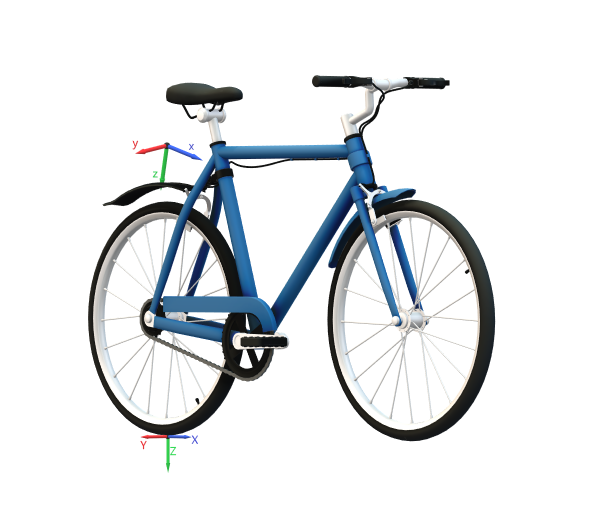
\includegraphics[width=0.7\textwidth]{images/whipple_axis.png}
    \caption{Bicycle with body fixed sensor axis x-y-z (B) and global axis XYZ (G). }
    \label{fig:bike_imu}
\end{figure}

Different orders of rotation affects the end configuration. For this study the intrinsic order Z-Y'-X'' is adopted which is equivalent to the extrinsic X-Y-Z (roll-pitch-yaw). The inverse rotation matrix that described the above rotation sequence is :
\begin{equation}
R_{xyz}=R_x(\phi)R_y(\theta)R_z(\psi)=\left(\begin{array}{ccc}{\cos \theta \cos \psi} & {\cos \theta \sin \psi} & {-\sin \theta} \\ {\cos \psi \sin \theta \sin \phi-\cos \phi \sin \psi} & {\cos \phi \cos \psi+\sin \theta \sin \phi \sin \psi} & {\cos \theta \sin \phi} \\ {\cos \phi \cos \psi \sin \theta+\sin \phi \sin \psi} & {\cos \phi \sin \theta \sin \psi-\cos \psi \sin \phi} & {\cos \theta \cos \phi}\end{array}\right)
    \label{eq:rotmat}
\end{equation}

where \ensuremath{\phi} is the angle of rotation around axis X, \ensuremath{\theta} is the angle of rotation around axis Y and \ensuremath{\psi} is the angle of rotation around axis Z. \Cref{eq:rotmat} maps a vector from the global system G to the body fixed system B. In order to estimate the euler angle offsets the bike was configured in two different ways to aligne the gravity vector with the z and x axis respectively.
The readings from the accelerometer are expressed in the sensor frame (B). \Cref{eq:firstIMU}  is used to solve for the euler angle offsets. Unfortunately the three equations have only two degrees of freedom so two configurations are required so as to solve for all three angles. 

 In the first, \ensuremath{i=1} and \ensuremath{\boldsymbol{g}_1=[ 0 \;\; 0 \;\; 1]^T }(see \cref{fig:config1}) (note that the vector of accelerations is normalized)  with \cref{eq:firstIMU} solving for \ensuremath{\theta} and \ensuremath{\phi}. The lack of any dependence on the yaw  angle is intuitive to understand since a rotation  around the z-axis is aligned with the gravitational field and accelerometers are completely insensitive to rotations about the gravitational field vector. Consequently in the second, \ensuremath{i=2} and \ensuremath{\boldsymbol{g}_2=[ -1 \;\;0\;\; 0 ]^T} which leads to   \cref{eq:firstIMU} solving for \ensuremath{\psi} and \ensuremath{\theta} (see \cref{fig:config2}).
 
 \begin{figure}
    \centering
    \begin{subfigure}[htbb]{0.48\textwidth}
        \centering
        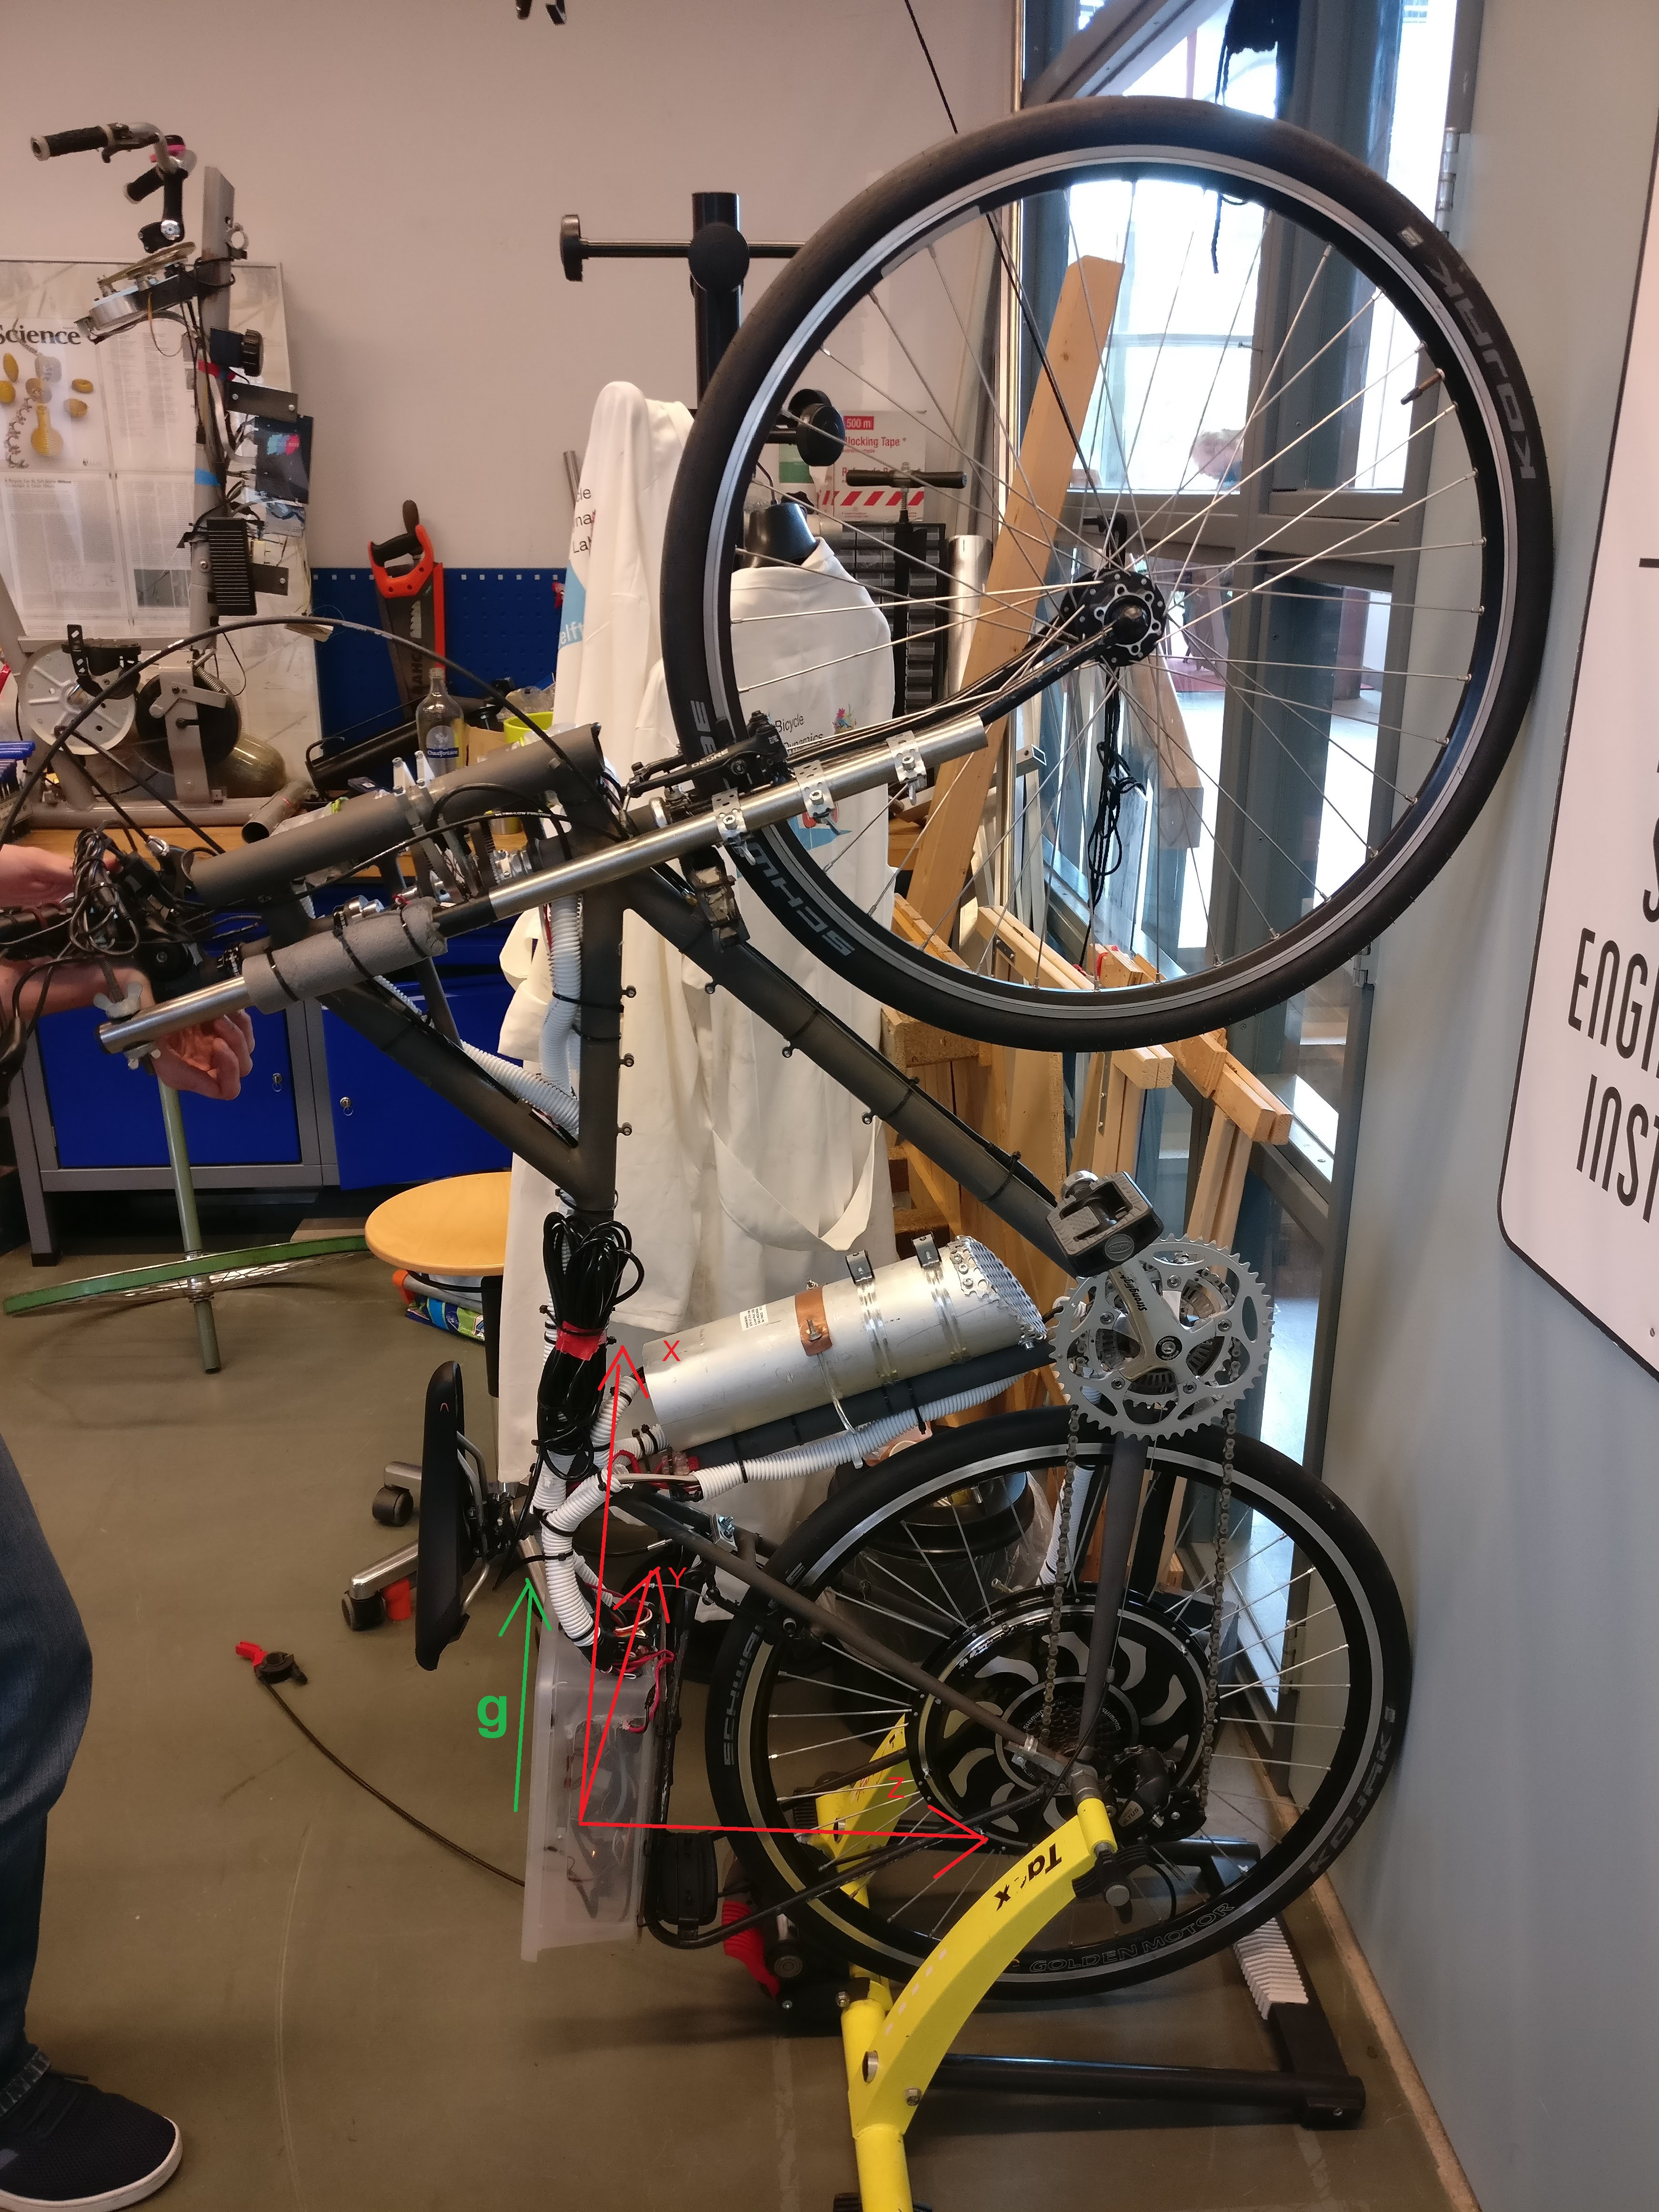
\includegraphics[width=\textwidth]{images/bike_upright.jpg}
        \caption{Configuration \ensuremath{i=1}}
        \label{fig:config1}
    \end{subfigure}
    \hfill
    \begin{subfigure}[htbb]{0.48\textwidth}
        \centering
        \includegraphics[width=\textwidth]{images/bike_vertical.png}
        \caption{Configuration \ensuremath{i=2}}
        \label{fig:config2}
    \end{subfigure}
    \caption{a) The bicycle's desired Z axis is aligned with the vector of gravitational acceleration. The bike was validated to be completely upright by the use of a calibrated commerical IMU (MTw Awinda). b) The bicycle's desired X axis is aligned with the vector of gravitational acceleration. The door was validated to be completely vertical by the use of a calibrated commerical IMU (MTw Awinda). \ensuremath{\mathbf{g}} is the vector measured by the accelerometer which oposite to the gravitational acceleration.}
 \end{figure}
 \begin{equation}
 \frac{\boldsymbol{G}_{i}^B}{\norm{\boldsymbol{G}_{i}^B}}=\left(\begin{array}{l}{G_{i x}^B} \\ {G_{i y}^B} \\ {G_{i z}^B}\end{array}\right)\frac{1}{\sqrt{{G_{i x}^B}^2+{G_{i y}^B}^2+{G_{i z}^B}^2}}=\boldsymbol{R}_{\mathit{xyz}(\phi_o,\theta_o,\psi_o)}\boldsymbol{g}_i
\label{eq:firstIMU}
 \end{equation}
 
Solving \cref{eq:firstIMU} for the angles we get :
\begin{align}
   & \phi_o=tan^{-1}\left(\frac{G_{1y}^B}{G_{1z}^B}\right)
   \label{eq:offset1}
   \\
   & \theta_o= tan^{-1}\left(\frac{G_{1 x}^B}{\sqrt{{G_{1 y}^B}^{2}+{G_{1 z}^B}^{2}}}\right) 
   \label{eq:offset2}
   \\
   & \psi_o = tan^{-1}\left(\frac{-G_{2 y}^B}{\sqrt{{G_{2 x}^B}^{2}+{G_{2 z}^B}^{2}}}\right)
   \label{eq:offset3}
\end{align}

From \crefrange{eq:offset1}{eq:offset3} the euler angle offsets calculated are inserted into rotation matrix \ensuremath{R_{\mathit{xyz}}}. The transpose of the result (\ref{eq:resultIMU}) is then used to transform the IMU measurements from the coordinate frame B to the coordinate frame G which is consistent with the linearized equations of motion defined in \cref{subsec:EOM}.

\begin{equation}
R_{\mathit{IMU}}=R_{\mathit{xyz}}^T(\phi_o,\theta_o,\psi_o)=\left(\begin{array}{ccc} 0.9939 & -0.006106 & -0.1105\\ 0.006069 & 1.0 & -0.000675\\ 0.1105 & 0 & 0.9939 \end{array}\right)
    \label{eq:resultIMU}
\end{equation}

\bibliography{report}

\end{document}

